\documentclass[twoside,10pt]{book}
\usepackage{amsmath, honstyle}				%Page style and numbering
\usepackage{setspace, enumerate,graphicx,amssymb}

%Put "\layout" in begin document to see the layout
\usepackage{layout}

%-------------------------------------------------------------------------------
%Changes sizes of the leftside margins so that, for odd pages, there's a larger margin on the right and a larger margin on the left for even pages
\setlength{\oddsidemargin}{7pt}
\setlength{\evensidemargin}{-23pt}
\setlength{\textwidth}{490pt}
\setlength{\textheight}{600pt}
\setlength{\topmargin}{0pt}
% Length to control the \fancyheadoffset and the calculation of \headline
% simultaneously
\newlength\FHoffset
\setlength\FHoffset{0cm}
\addtolength\headwidth{2\FHoffset}
\fancyheadoffset{\FHoffset}

%-------------------------------------------------------------------------------

%-------------------------------------------------------------------------------
%Some stuff I've added
\usepackage{amsthm}
\usepackage{mathtools}
\usepackage{placeins} %for \FloatBarrier
\usepackage{comment} %Allow use of the \begin{comment} environment
\SetSymbolFont{stmry}{bold}{U}{stmry}{m}{n} %for bold math symbols
\usepackage{cancel} %for strikethrough

%Stuff Paul had
\usepackage{hyperref, tocvsec2} %Hyperlinks document and lets me set the depth of the toc
\usepackage[title,titletoc]{appendix} %gives appendices environment and adds 'Appendix' into toc
\settocdepth{section} %set depth of toc upto sections
%%%%%%%%%\onehalfspacing
\numberwithin{equation}{chapter} %numbers reset for each chapter
\numberwithin{figure}{chapter}

%Packages
\usepackage{algorithm} %for writing pseudoalgorithms
\usepackage{algpseudocode} %for writing pseudoalgorithms
\usepackage{multirow} %for tables
\usepackage{graphicx}
\usepackage{hyperref}
\graphicspath{{Figures/}}
\newcommand{\figscale}{0.4}
\usepackage{dsfont} %for mathds fonts

%Including Python Code
\usepackage[dvipsnames]{xcolor}
\usepackage{listings} %for including Python code
\usepackage{lstautogobble} % For cleaning code spaces
% Bash (terminal) style
\lstdefinestyle{bash}{
    language=bash,
    basicstyle=\footnotesize\ttfamily\color{white},
    backgroundcolor=\color{black},
    commentstyle=\color{green}
}

% Python style
\lstdefinestyle{python}{
    language=Python,
    basicstyle=\footnotesize\ttfamily\color{white},
    backgroundcolor=\color{darkgray},
    keywordstyle=\color{Cerulean}\bfseries,
    commentstyle=\color{YellowGreen},
    stringstyle=\color{yellow}
}

% C++ style
\lstdefinestyle{cpp}{
    language=C++,
    basicstyle=\footnotesize\ttfamily\color{white},
    backgroundcolor=\color{darkgray},
    keywordstyle=\color{Cerulean}\bfseries,
    commentstyle=\color{YellowGreen},
    stringstyle=\color{yellow}
}

% Setting default style and settings
\lstset{
  style=bash,
  upquote=true,
  numbers=none,
  breaklines=true,
  breakatwhitespace=false,
  breakautoindent=true,
  keepspaces=true,
  showspaces=false,
  showstringspaces=false,
  showtabs=false,
  tabsize=2,
  columns=fullflexible,
  autogobble=true,
  abovecaptionskip=0.5cm,
  belowcaptionskip=0.5cm
}

% Additional Commands
\newcommand{\tsim}{$\sim$}
\newcommand{\tlangle}{$<$}
\newcommand{\trangle}{$>$}

%-------------------------------------------------------------------------------

%-------------------------------------------------------------------------------
%Layouts
\newtheorem{theorem}{Theorem}[section]
\newtheorem{lemma}[theorem]{Lemma}
\newtheorem{claim}[theorem]{Claim}
\newtheorem{proposition}[theorem]{Proposition}
\newtheorem{corollary}[theorem]{Corollary}
\newtheorem{remark}[theorem]{Remark}
\newtheorem{definition}[theorem]{Definition}
\newtheorem{example}[theorem]{Example}
%-------------------------------------------------------------------------------
\begin{document}
	%\layout
	\pagenumbering{roman}
	\setcounter{page}{1}
	\begin{titlepage}
\hoffset = .25in

\begin{center}

{\huge \bf Workflow Notes}

\rule{\linewidth}{0.8mm} \vspace{2.5cm}
\end{center}
\begin{flushright}

\emph{\large May 17th 2020:}

 \LARGE{ Hwan Goh} \vspace{10cm}

\end{flushright}

\end{titlepage}


	\newpage\null\thispagestyle{empty}\newpage
	\paragraph{ \vspace{3.5cm}}\begin{center}\end{center}


%: --------------------------------------------------------------
%:                  FRONT MATTER:  Abstract
% ---------------------------------------------------------------

\noindent \textbf{ {\Large Abstract}}

\paragraph{}
Notes detailing my workflow using Vim and i3wm. Also details emulation on
Windows.

%: -------------------------------------------------------------
%:                  END:  Abstract
% --------------------------------------------------------------

\newpage
\paragraph{ \vspace{3.5cm}}\begin{center}\end{center}
% --------------------------------------------------------------
%:                           Content
% --------------------------------------------------------------

\tableofcontents

\chapter{Vim} \label{ChapVim}
\pagenumbering{arabic}
\setcounter{page}{1}

%===============================================================
\section{Vim Tips and Tricks}
%===============================================================
Some good references are \cite{chang2018vim,toomey2015mastering}. A more
advanced tutorial that I haven't watched yet is \cite{chang2020vim}. A document
on effective text editing written by the creator of Vim can be found at
\cite{moolenaar2000seven}.
\begin{enumerate}
    \item In Linux based systems, put `setxkbmap -option "caps:escape' into
        ~/.bashrc to map the caps lock key to escape.
    \item To set Vim as your default text editor, use `sudo update-alternatives
        --config editor'.  \item Suppose the cursor is in the middle of a word.
        Whilst `cw' and `dw' will change/delete until the end of the word, `ciw'
        and 'diw' to change or delete the whole word, thereby not requiring you
        to move the cursor to the beginning of the word first.
    \item To reformat a paragraph, use `gq'. Reformatting includes enforcing the
        wrap limit which can be set in your vimrc with `set tw=\tlangle
        number\trangle'. Other options can be se such as indentation. Note that
        this command requires a minimum of two lines, so you'll need to at least
        use `gqj' and at most use `gjG' for the rest of the document under the
        line currently under the cursor.
    \item Use `m\tlangle key\trangle to set a mark to \tlangle key\trangle then
        \tlangle key\trangle to jump to it.  Note that if you set it to the
        capitalized version of \tlangle key\trangle then the jumping can occur
        between buffers. To see your list of marks, use `:mark'.
    \item Use `"\tlangle key\trangle' then an action like `y' or `d' to store
        text in the \textit{register} \tlangle key\trangle. Then use `"\tlangle
        key\trangle p' to paste it. Note that using `d' will automatically store
        it in the register at register x and `p' will automatically paste
        whatever is in register `x'.  Use `:reg' to see the register list.
    \item Use `f\tlangle key\trangle' to forward search for \tlangle
        key\trangle. To backwards search, use `F\tlangle key\trangle'. To repeat
        the search, use `;'.
    \item The `t' stands for `til'. For example, `dt=' will delete up to and not
        including an = sign.  \item The `*' can be used to search for the word
        under cursor.
    \item `J' is used to join the line below to the line currently under the
        cursor. This is useful for reformatting improperly wrapped lines but in
        general `gq' is more useful for this purpose.
    \item `zt' or `z<CR>' will put the line under the cursor to the to of the
        window. `z.' will put the line to the center of the window and `z-' will
        put it to the bottom of the window.
    \item `z=' will give spelling suggestions for the word under the cursor.
    \item `[s' and `]s' to cycle backwards and forwards through misspelled words.
    \item Use `g\$' to go to the end of an unwrapped line.
    \item If you type a long line of text in insert mode, this counts as one
        action. Therefore, if you press undo, the whole line will be deleted. To
        break the undo chain, use \tlangle c-g\trangle u while in insert mode.
        Alternatively, you could map space to \tlangle c-g\trangle u so that the
        undo chain is broken whenever a space is added in insert mode:\\
        inoremap \tlangle Space\trangle \tlangle Space\trangle \tlangle
        c-g\trangle u
    \item Use the accent `\tlangle shift+6\trangle' in insert mode to move to
        the first non-white space character in the line.
    \item Use `\%' while your cursor is over a parenthesis, square or curly
        bracket to move to the corresponding open/closing parenthesis or
        bracket.
    \item Use `:ls' to see the list of buffers then `:b' and the number to
        select one. A useful mapping for this process is:\\ nnoremap \tlangle
        leader\trangle b:ls\tlangle cr\trangle:b\tlangle space\trangle
    \item Use `\tlangle number\trangle +\tlangle c-6\trangle' to switch to numbered buffer.
    \item Use `\tlangle c-f\trangle' in command line mode to view the command history in a
        buffer.
    \item In general, all yank, change or delete actions such as `y, c, d, x'
        etc will register the text object into the "" register. However, any
        yank action will also register the text object into the "0 register and
        any delete or change action will register the text object into the "-
        register.
    \item Use `s' or `S' to substitute. This is useful when you want to replace
        one letter with multiple letters.
    \item When using search `/\tlangle word\trangle', you can use \tlangle c-g
        \trangle and \tlangle c-t\trangle to cycle through them without
        confirming your search with \tlangle CR\trangle.
    \item Use `\tlangle c-r\trangle' in command line mode to paste from the
        register.
    \item Use `\tlangle c-r\trangle' in insert mode to paste from the register.
    \item Use \tlangle c-w\trangle N in a Vim terminal to switch to normal mode, which allows
        you to navigate as if you were in Vim.
    \item Use `\tlangle c-z\trangle' to suspend Vim and return to shell. Use `fg'
        in shell to resume the suspended program. You can also use
        \begin{lstlisting}
            stty susp undef
            bind '"\C-z":"fg\015"'
        \end{lstlisting}
        in your bashrc to, overall, set `\tlangle c-z\trangle' to toggle a
        suspended progran.
    \item Using `ctags -R' in terminal creates a tag file. Then, in vim, use
        `\tlangle c-$]$ \trangle' while the cursor is over a function name to
        jump to the code defining the function. You can also add the following
        shortcut to your vimrc:
        \begin{lstlisting}
            command! MakeTags !ctags -R .
        \end{lstlisting}
        so that tags can be created from the command line within Vim.
        Note that you need to add
        \begin{lstlisting}
            set tags=tags;/
        \end{lstlisting}
        to your vimrc so that ctags will check the current folder for tags file
        and keep going one directory all the way to root folder. See
        \cite{ben2011ctags} for more details.
\end{enumerate}

%===============================================================
\section{Plugin Management}
%===============================================================
The first part of this section follows \cite{neil2010synchronizing}. First, we
work towards turning ~/.vim into a git repository:
\begin{enumerate}
    \item Move \tsim/.vimrc into \tsim/vim.
    \item When vim boots, it's still going to look for .vimrc in the home
        directory. To ensure that it looks for vimrc in the \tsim/.vim
        directory, we can create a symbolic link to that file using `ln -s
        \tsim/.vim/vimrc \tsim/.vimrc'.  \item Make \tsim/.vim into a git
        repository.
\end{enumerate}
An issue now is if you install a plugin that itself is a git repository, you
lose the version-control capabilities of that plugin. To circumvent this issue,
we use a plugin manager; in this case \textit{Pathogen}.\\

%---------------------------------------------------------------
\subsection{Pathogen} \label{SecPathogen}
%---------------------------------------------------------------
The pathogen plugin makes it possible to cleanly install plugins as a bundle.
Rather than having to place all of your plugins side by side in the same
directory, you can keep all of the files for each individual plugin together in
one directory (see video from first link for example). This makes installation
more straightforward, and also simplifies the tasks of upgrading and even
removing a plugin if you decide you no longer need it since they are carefully
segregated from each other. For a good tutorial on Pathogen, see
\cite{lafourcade2014how}.\\

Following the readme on the repo at \cite{pope2009pathogen}, to install Pathogen
do the following:
\begin{enumerate}
    \item Run in terminal:\\
        mkdir -p \tsim/.vim/autoload \tsim/.vim/bundle \&\& \ \\ curl -LSso
        \tsim/.vim/autoload/pathogen.vim https://tpo.pe/pathogen.vim
    \item Add the following to your vimrc:
        execute pathogen\#infect()
\end{enumerate}
Now any plugins you wish to install can be extracted to a subdirectory under
~/.vim/bundle, and they will be added to the 'runtimepath'. For example, to
install "sensible.vim", simply run: "cd ~/.vim/bundle \&\& \ git clone
https://github.com/tpope/vim-sensible.git".

%---------------------------------------------------------------
\subsection{Submodules: Installing Git Repositories Within Git Repositories}\label{SecSubmodules}
%---------------------------------------------------------------
This section follows \cite{neil2010synchronizing}. Now that we can install
plugins via Pathogen, let's see how we preserve the version control capabilities
of our plugins. As a worked example, let us install the \textit{Vimtex} plugin:
\begin{enumerate}
    \item cd \tsim/.vim
    \item Now to clone a git repository into the bundle directory, use:\\ git
        submodule add https://github.com/lervag/vimtex.git bundle/vimtex
\end{enumerate}
Now, to upgrade this plugin, use:
\begin{enumerate}
    \item cd \tsim/.vim/bundle/vimtex
    \item git pull origin master
\end{enumerate}
To update ALL of your plugins, use:
\begin{enumerate}
    \item cd \tsim/.vim
    \item git submodule foreach git pull origin master
\end{enumerate}
%---------------------------------------------------------------
\subsection{Importing Your Vim Configuration and Plugins To a New Machines}
%---------------------------------------------------------------
One of the main benefits of version controlling your Vim configuration and
plugins is the ease of which they can be imported into a new machine. To do so,
use the following:
\begin{enumerate}
    \item cd \tsim
    \item git clone \tlangle git repo url\trangle \tsim/.vim
    \item ln -s \tsim/.vim/vimrc \tsim/.vimrc
    \item cd \tsim/.vim
    \item git submodule init
    \item git submodule update
\end{enumerate}
%---------------------------------------------------------------
\subsection{Vim-plug}
%---------------------------------------------------------------
Whilst Pathogen is the most basic plugin manager, there are limitations when
porting your setup to a new machine:
\begin{enumerate}
    \item When you run git submodule update, you'll pull the latest versions of
        the plugins from their respective repositories. So unless you've noted
        down somewhere all the commit IDs for your favourite version of each
        plugin, your overall plugin collection cannot be preserved when porting
        to a new machine.
    \item Suppose one of the plugins is no longer being maintained by the owner
        and suppose also that you've made your own changes to the plugin. If you
        were to pull your configuration on a new machine, you will pull the
        latest version of the plugin; that is your changes will not be ported.
        Further, on your own repository for your configuration, the directories
        containing the plugins will be treated as repositories. Unless you
        manually install the plugins, there is no way to preserve your changes
        onto Github.
\end{enumerate}
The plugin manager Vim-plug \cite{junegunn2014vimplug} has a solution to the
first problem. This plugin manager is extremely simple to use:
\begin{enumerate}
    \item Run in terminal:\\
        curl -fLo \tsim/.vim/autoload/plug.vim --create-dirs \
        https://raw.githubusercontent.com/junegunn/vim-plug/master/plug.vim
    \item In your vimrc, add the line:\\
        call plug\#begin('\tsim/.vim/plugged')
    \item To include a plugin you wish to install under the line above, in your
        vimrc add the following line:\\
        Plug 'https://github.com/lervag/vimtex.git'
    \item Under `Plug \tlangle url \trangle' of your last plugin, in your vimrc
        add the following line:\\
        call plug\#end()
    \item Reload your vimrc and use the command `:PlugInstall' while in vim. Now
        all your plugins are installed.
\end{enumerate}
Now to preserve the versions of your plugin:
\begin{enumerate}
    \item In Vim, run the command `:PlugSnapshot! \tlangle filename \trangle.vim'.
    \item To restore the state of your plugins, in vim run the command:\\
        :source \tsim/.vim/\tlangle filename \trangle.vim\\
        or, in terminal:\\
        vim -S \tsim/.vim/\tlangle filename \trangle.vim
\end{enumerate}
See the bradagy's answer in the reddit post \cite{bradagy2018remember}. To port
your configuration to a new machine:
\begin{enumerate}
    \item cd \tsim
    \item git clone \tlangle git repo url \trangle \tsim/.vim
    \item cd \tsim/.vim/vimrc
    \item :PlugInstall
    \item :source \tsim/.vim/\tlangle filename \trangle.vim
\end{enumerate}
To uninstall plugins:
\begin{enumerate}
    \item Delete `Plug \tlangle url \trangle' line from your vimrc
    \item :PlugClean
\end{enumerate}
%===============================================================
\section{Native Plugin Management} \label{SecNativePluginManagement}
%===============================================================
Vim-plug provides a solution to the first of the two issues mentioned in the
previous section, but not the second. To address the second issue, we can use
Vim's native plugin management system to install a plugin and delete the .git
repository. That way, we can track the files and any changes in our own git
repository. This section follows \cite{shapeshed2019vim}. For a more
detailed explanation, see \cite{manasthakur2020managing} or \cite{ryder2018attack}.\\

The package feature of Vim 8 follows a pathogen-like model and adds the plugins
found inside a custom-path \tsim/.vim/pack/ to Vim's runtime path. You can check
the version of Vim installed using `vim --version'. To install using this native
feature, we use the following steps:
\begin{enumerate}
    \item mkdir -p \tsim/.vim/pack/plugins/start/
    \item cd \tsim/.vim/pack/plugins/start/
    \item git clone \tlangle url\trangle or git submodule add \tlangle url
        \trangle
\end{enumerate}
and that's it! To remove a plugin, simply remove its directory: rm -r
\tsim/.vim/pack/plugins/start/\tlangle plugin\_directory\_name \trangle if the
plugin was cloned. Or, if it was added as a submodule, use:
\begin{enumerate}
    \item git submodule deinit vim/pack/shapeshed/start/\tlangle plugin\_directory\_name \trangle
    \item git rm vim/pack/shapeshed/start/\tlangle plugin\_directory\_name \trangle
    \item rm -Rf .git/modules/vim/pack/shapeshed/start/\tlangle plugin\_directory\_name \trangle
\end{enumerate}
To import your vim configuation and plugins to your new machine, simply use the
same steps as required for Pathogen:
\begin{enumerate}
    \item cd \tsim
    \item git clone \tlangle git repo url\trangle \tsim/.vim
    \item ln -s \tsim/.vim/vimrc \tsim/.vimrc
    \item cd \tsim/.vim
    \item git submodule init
    \item git submodule update
\end{enumerate}
and also, to update all your plugins, you again use
\begin{enumerate}
    \item cd \tsim/.vim
    \item git submodule foreach git pull origin master
\end{enumerate}
If you have your own plugins that are not cloned from external repositories
(i.e. you've written your own .vim files), you can simply create a directory
~/.vim/plugin and copy your plugins into there.\\

In conclusion, although Pathogen seems to be the most cumbersome, it could be
the case that the servers do not have Vim 8 installed and so the native plugin
manager will not work nor do they allow Vim-plug to install plugins. In such a
case, Pathogen is your best bet.

%===============================================================
\section{Vimtex}
%===============================================================
This section discusses the Vimtex \cite{lervag2015vim} plugin. See also the
vimways article \cite{woodruff2019latex} for a good overview.  To install MikTex
into Linux, run ``sudo apt-get install texlive-full''.

%---------------------------------------------------------------
\subsection{Installing and Running Vimtex}
%---------------------------------------------------------------
Assuming you are using the Pathogen plugin manager and version controlling your
~/.vim directory, follow the steps used in Section \ref{SecSubmodules}. Then use
`:Helptags' which is Pathogen's method for generating help tags. With this, we
can use `:h vimtex' to see the manual for Vimtex. To confirm that the plugin
works, type ":VimtexInfo" to see a summary of the tex file.
%---------------------------------------------------------------
\subsection{Compiling a Tex File}
%---------------------------------------------------------------
The following commands are useful:
\begin{itemize}
    \item :VimtexCompile \# this is a continuous compiler meaning that everytime
        you save with ":w" it will automatically compile
    \item :VimtexStop \# this stops the continuous compiler
    \item :VimtexCompileSS \# this is a single shot compiler. Note that you have
        to save your file first \item :VimtexClean \# Cleans auxiliary files
        generated in compilation process
\end{itemize}
I set the following mappings in my vimrc:
\begin{lstlisting}
autocmd FileType tex nnoremap <F5> :VimtexView<CR>
autocmd FileType tex inoremap <F5> <Esc> :VimtexView<CR>
autocmd FileType tex nnoremap <F6> :w! <bar> :VimtexCompileSS<CR>
autocmd FileType tex inoremap <F6> <Esc> :w! <bar> :VimtexCompileSS<CR>
\end{lstlisting}
Here are some useful commands I use in my vimrc:
\begin{lstlisting}
" Avoids opening an empty .tx file only to have vimtex recognize it as plain Tex rather than Latex
    let g:tex_flavor = 'latex'

" Use folding. Use zx to unfold and zX to fold all
    let g:vimtex_fold_enabled = 1

" Toggle Error Window On and Off
    autocmd FileType tex map <F4> \le

" Shortcut for Compiling and Viewing PDF
    autocmd FileType tex nnoremap <F5> :VimtexView<CR>
    autocmd FileType tex inoremap <F5> <Esc> :VimtexView<CR>
    autocmd FileType tex nnoremap <F6> :w! <bar> :VimtexCompileSS<CR>
    autocmd FileType tex inoremap <F6> <Esc> :w! <bar> :VimtexCompileSS<CR>

" VimtexClean on exit
  augroup vimtex_config
    au!
    au User VimtexEventQuit call vimtex#compiler#clean(0)
  augroup END
\end{lstlisting}
And here are some useful mappings for creating common math related LaTeX tex
objects:
\begin{lstlisting}
" Teleportation!
    autocmd FileType tex inoremap <Space><Space> <Esc>/<++><CR>"_c4l

" Inline Stuff
    autocmd FileType tex inoremap ;mm $$<++><Esc>5ha
    autocmd FileType tex inoremap ;bf \textbf{}<++><Esc>6hf}i
    autocmd FileType tex inoremap ;it \textit{}<++><Esc>6hf}i
    autocmd FileType tex inoremap ;bfs \boldsymbol{}<++><Esc>6hf}i
    autocmd FileType tex inoremap ;ct \cite{}<++><Esc>6hf}i
    autocmd FileType tex inoremap ;lb \label{}<++><Esc>6hf}i
    autocmd FileType tex inoremap ;rf \ref{}<++><Esc>6hf}i
    autocmd FileType tex inoremap ;erf (\ref{})<++><Esc>7hf}i

" Environments
    autocmd FileType tex inoremap ;itm \begin{itemize}<CR><CR>\end{itemize}<CR><++><Esc>2kA\item<Space>
    autocmd FileType tex inoremap ;enu \begin{enumerate}<CR><CR>\end{enumerate}<CR><++><Esc>2kA\item<Space>
    autocmd FileType tex inoremap ;aln \begin{align}<CR><CR>\end{align}<CR><++><Esc>2kA

" Math Environments
    autocmd Filetype tex inoremap ;def \begin{definition}<CR><CR>\end{definition}<CR><++><Esc>2kA
    autocmd Filetype tex inoremap ;thm \begin{theorem}<CR><CR>\end{theorem}<CR><++><Esc>2kA
    autocmd Filetype tex inoremap ;lem \begin{lemma}<CR><CR>\end{lemma}<CR><++><Esc>2kA
    autocmd Filetype tex inoremap ;cor \begin{corollary}<CR><CR>\end{corollary}<CR><++><Esc>2kA
    autocmd Filetype tex inoremap ;prp \begin{proposition}<CR><CR>\end{proposition}<CR><++><Esc>2kA
    autocmd Filetype tex inoremap ;prf \begin{proof}<CR><CR>\end{proof}<Esc>1kA

" Math Stuff
    autocmd Filetype tex inoremap ;T ^\mathrm{T}
    autocmd FileType tex inoremap ;sd _{}<++><Esc>6hf}i
    autocmd FileType tex inoremap ;su ^{}<++><Esc>6hf}i
    autocmd FileType tex inoremap ;frc \frac{}{<++>}<++><Esc>12hf}i
    autocmd FileType tex inoremap ;mbb \mathbb{}<++><Esc>6hf}i
    autocmd FileType tex inoremap ;lrp \left(\right)<++><Esc>12hf(a
    autocmd FileType tex inoremap ;lrs \left[\right]<++><Esc>12hf[a
    autocmd FileType tex inoremap ;lrn \left\lVert\right\rVert<++><Esc>15hi<Space>
\end{lstlisting}

%---------------------------------------------------------------
\subsection{Forward and Backwards Searching with Synctex}
\label{SecFwdBckwdSynctex}
%---------------------------------------------------------------
This section follows \cite{gunther2014vimtex}. For this, you will need a Vimtex
server which allows you to do forward and backward to navigate between
corresponding sections of the tex file and the pdf. You will also need the pdf
viewer \textit{Zathura}. To install, simply use `sudo apt-get install zathura'.
Then, in your vimrc, add the following line `let g:vimtex\_view\_method =
'zathura''.\\

Following \cite{lerner2004enable}, to install just use `sudo apt-get install
vim-gnome'. Finally, to edit a tex file with navigation capabilities:
\begin{enumerate}
    \item In the directory containing the tex file, use:\\
        vim --servername \tlangle servername\trangle \tlangle texfile\trangle.tex
    \item While in tex file, to jump to the text on the pdf corresponding to the
        line under your cursor, use:\\
        \tlangle leader\trangle lv
    \item Move your mouse cursor over some text on the pdf. Then, to jump to
        corresponding text on the tex file, use:\\
        Ctrl + left-click
\end{enumerate}
Note that \tlangle leader\trangle lv forward search works without the Vim
server; it's the backwards search that requires the Vim server.\\

Note that as of at least July 1st 2021, vim-gnome no longer exists.
Instead, use vim-gtk which can be installed with `sudo apt-get install
vim-gtk'.

%---------------------------------------------------------------
\subsection{Other Useful References}
%---------------------------------------------------------------
\begin{itemize}
    \item Good article overviewing Vimtex \cite{woodruff2019latex}
    \item Nice compilation of Vimtex commands \cite{gunther2014vimtex}
    \item Quick guide on the basics of Vimtex \cite{jdhao2019complete}
    \item For a comparison with other Vim LaTeX plugins \cite{lervag2015vim}
    \item Some useful mappings such as the teleportation trick
        \cite{smith2016my, smith2017start}.
    \item Note-taking using Vim and LaTeX for math lectures \cite{castel2019how}
    \item Vim and LaTeX on MacOS \cite{dyke2020getting}
\end{itemize}

%===============================================================
\section{IPython}
%===============================================================
The following mapping may prove useful for starting an IPython terminal in
Vim:\\
\begin{lstlisting}
nnoremap <leader>P :botright vertical terminal ipython --no-autoindent<CR><C-w><left>
\end{lstlisting}

%---------------------------------------------------------------
\subsection{sendtowindow Plugin}
%---------------------------------------------------------------
When coding in Python with a Vim terminal on the side running IPython, I use the
\textit{sendtowindow} plugin \cite{KKPMW2016send} to send lines of code to the
terminal. See \cite{KKPMW2019send} for a Reddit post from the author discussing
the plugin. It's a very simple plugin that allows the use of vim motions to move
lines of text to terminals left, right, above or below the Vim window. I use the
following maps:\\
\begin{lstlisting}
let g:sendtowindow_use_defaults=0
nmap ,sr <Plug> SendRight
xmap ,srv <Plug> SendRightV
nmap ,sl <Plug> SendLeft
xmap ,slv <Plug> SendLeftV
nmap ,su <Plug> SendUp
xmap ,suv <Plug> SendUpV
nmap ,sd <Plug> SendDown
xmap ,sdv <Plug> SendDownV
\end{lstlisting}
Note that these mappings must not be noremaps (mappings that are non-recursive). For an
explanation on why this is the case, please see \cite{justrajdeep2018please}.
Any one of these mappings will specify to either send some text in normal mode
or in visual mode. When in normal mode, to specify which text to send, use the
usual Vim movements. For example, `,sr\$' will send from the cursor to the end
of the line to the window on the right. However, if you are in the middle of a
line, it may become tedious having to first go to the beginning of the line and
having to type `\$'. Therefore, we can define line objects using the following
maps:
\begin{lstlisting}
onoremap <silent> <expr> - v:count==0 ? ":<c-u>normal! 0vg_<CR>" : ":<c-u>normal! V" . (v:count) . "jk<CR>"
onoremap <silent> <expr> i- v:count==0 ? ":<c-u>normal! ^vg_<CR>" : ":<c-u>normal! ^v" . (v:count) . "jkg_<CR>"
\end{lstlisting}
With '-' alone the indentation is left intact and 'i-' is without indentation.
So, for example, `,sr-' will send the line under the cursor to the window on
the right with indentation and `,sr8-' will send four lines under the cursor to
the window on the right with indentation. Note that this is important for Python as if you try
send a for loop with `i-' and leave out the indentation, then it may not run.\\

I have extended the plugin with SendTextToTerminalRight command and SendVariableRight()
and SendMarkedSectionRight() functions (I've also coded for the other three directions as
well). Using these, we can send clear, \%reset and run code commands as well as
variable and marked sections of code to the IPython terminal.
\begin{lstlisting}
" sendtowindow for IPython in Vim Terminal: clear, reset, run code, run variable, run marked section
    noremap ,sL :SendTextToTerminalRight clear<CR>
    noremap ,sD :SendTextToTerminalRight %reset -f<CR>
    noremap ,sR :w!<CR>:SendTextToTerminalRight run <c-r>%<CR>
    nmap ,sV <Plug>SendVariableRight
    nmap ,sM <Plug>SendMarkedSectionRight
\end{lstlisting}
For the map that runs the Python code, we leverage the fact that
`\tlangle c-r\trangle' in command mode will prime pasting from the register and
\% in the register stores the file name.\\

The SendMarkedSectionRight() function has been coded such that the section must
be marked with `x' on the top of the section and `z' on the bottom.  The plugin
vim-signature \cite{kshenoy2015signature} may come in handy for manipulating the
marks. In particular, the plugin displays marks and the command `dm\tlangle mark
name\trangle' deletes the mark; so `dmq' above deletes the mark called `q'.

%---------------------------------------------------------------
\subsection{Slimux plugin}
%---------------------------------------------------------------
There are many plugins that allow interaction between Vim and tmux. For example,
there is Vim-Slime \cite{jpalardy2012slime} and Vimux \cite{benmills2009vimux}.
The one I use is Slimux \cite{esamattis2015slimux}. There is a blog post about
it here \cite{suuronen2012slimux}. As discussed in the blog post, Slimux differs
from Vimux in that it is more disjoint from tmux. In particular, Vimux will
create a pane on which you must run your commands whereas Slimux allows you to
select the pane you wish to use. Also, unlike Vim-Slime, you do not need to
manually type in the pane to select it; in Slimux an interactive prompt is
given. It's also worth noting that Vim-Slime supports many terminal multiplexers
such as GNU Screen, kitty and Vim's native terminal.\\

However, with Slimux, there is an issue with sending commands to IPython where the
indentation is constantly carried over \cite{kmARC2015indentationerror}. There
are three proposed fixes
\cite{lotabout2017remove,karadaharu2016add,zcesur2018fix}. The first modifies
python.vim, the second modifies both slimux.vim and python.vim by implementing
IPython's cpaste function and the third modifies a single line of slimux.vim.
Since the repo owner hasn't pulled any of these fixes, I opted for the third fix
which requires changing line 328 of slimux.vim in the SlimuxSendCode() function:
\begin{lstlisting}
let b:code_packet["text"] = a:text
\end{lstlisting}
to:
\begin{lstlisting} let
b:code_packet["text"] = "\e[200~" . a:text . "\e[201~\r\r.
\end{lstlisting}
There is also an issue with the SlimuxSendKeys() function. This function sends
keys to the terminal using the `tmux send-keys' syntax. A simple fix is to
change line 228 of slimux.vim from
\begin{lstlisting}
call system(g:slimux_tmux_path . ' send-keys -t " . target . " " . keys)
\end{lstlisting}
to
\begin{lstlisting}
call system(g:slimux_tmux_path . " send-keys -t " . target . " " . keys)
\end{lstlisting}
It's surprising that this small typo went unnoticed. Note that this repository has not
been updated in years and so all pull requests have not been fulfilled.
Therefore, if you wish to track the fixes you've made, you may want to install
the plugin manually so that it does not follow the original repository. This was
disussed in Section \ref{SecNativePluginManagement}.\\

I use the following mappings:
\begin{lstlisting}
" Primer for Vim motions to select text to be sent
    nmap ,t <Plug>SlimuxREPLSendWithMotion

" Send text selected in visual mode
    vnoremap ,t :SlimuxREPLSendSelection<CR>

" Send terminal commands
    nnoremap ,tX :SlimuxShellPrompt<CR>
    nnoremap ,tT :SlimuxShellRun<Space>
    nnoremap ,tE :SlimuxShellRun exit<CR>

" Send keys using the 'tmux send-keys' syntax
    nnoremap ,tK :SlimuxSendKeys<Space>
    nnoremap ,tC :SlimuxSendKeys<Space>c-c<CR>

" Slimux for IPython in tmux terminal : IPython, clear, reset, run code, run variable, run marked section
    nnoremap ,tP :SlimuxShellRun ipython<CR>
    nnoremap ,tL :SlimuxShellRun clear<CR>
    nnoremap ,tD :SlimuxShellRun %reset -f<CR>
    nnoremap ,tR :w!<CR>:SlimuxShellRun run <c-r>%<CR>
    nmap ,tV <Plug>SlimuxREPLSendVariable
    nmap ,tM <Plug>SlimuxREPLSendMarkedSection
\end{lstlisting}
where SlimexShellRun awaits a command to send to shell and SLimuxSendKeys sends
key inputs using the 'tmux send-keys' syntax. The SlimuxREPLSendWithMotion was
not part of the original slimux plugin. My code is as follows:
\begin{lstlisting}
function! s:GetTextWithMotion(type)
  let s:saved_registert = @t

  " Obtain wanted text
  if a:type ==# "char"
    keepjumps normal! `[v`]"ty
    call setpos(".", getpos("']"))
  elseif a:type ==# "line"
    keepjumps normal! `[V`]$"ty
    call setpos(".", getpos("']"))
  endif
  let text = @t

  " Restore register
  let @t = s:saved_registert

  return text
endfunction

function! s:SlimuxREPLSendWithMotion(type)
   let text = s:GetTextWithMotion(a:type)
   call SlimuxSendCode(text)
endfunction

nnoremap <silent> <Plug>SlimuxREPLSendWithMotion :<C-U> set operatorfunc=<SID>SlimuxREPLSendWithMotion<CR>g@
\end{lstlisting}
The `g@' sets the mark `[' at the beginning of the motion and `]' at the end of
the motion. This can then be leveraged in functions. The `@' in the context of
functions refers to the register.

%---------------------------------------------------------------
\subsection{Other Useful References}
%---------------------------------------------------------------
\begin{itemize}
    \item A good Reddit thread on workflow with Vim and IPython can be found at
        \cite{abdeljalil732020anyone}. Note that the majority of the responses
        indicate that they use vim-slime and tmux.
    \item The vim-tmux-runner plugin \cite{toomey2013tmuxrunner} may be worth checking out.
    \item The vim-ipython-cell plugin \cite{hanschen2019ipython} may be worth
        checking out. There is a reddit post \cite{hanschen2019reddit} by the
        author on this plugin. Note that this plugin is leverages vim-slime.
        According to the author, the main contribution of this plugin is that it
        provides many ways to define and run cells, even using Vim marks.
    \item Another lightweight workflow can be found in
        \cite{hornung2019boosting}. For this, you will need three plugins: Vimux
        \cite{benmills2009vimux}, vim-pyShell \cite{hornung2019pyShell} and
        vim-cellmode \cite{julienr2016vimcellmode}. However, I have trouble
        getting this to work. Starting and stopping a pyShell session works fine
        as well as sending one line of code, but I have issues sending over
        cells.
\end{itemize}

%==============================================================================
\section{Autocompletion with YCM}
%==============================================================================
When deciding between \emph{You Complete Me (YCM)} \cite{ycmcore2017ycm} and
\emph{Conquer of Completion (CoC)} \cite{neoclide2020conquer}, I found the
following the discussion in \cite{desmap2020ycmvscoc} where a maintainer of YCM
details the design philosophy of YCM in the comments. Specifically, one of the
maintainers (puremourning) states that YCM prioritizes consistency, testing,
stability and performance over a range of functions such as snippet support of
insertion of parentheses. This appeals to me because honestly all I want is to
be able to jump to definition. Finally, as of writing this, I prefer to
out-source error checking to the compiler and linting to some external linting
program. Basically, I want my text-editor to just edit text and help me navigate
my code. With this in mind, YCM seems ideal as you can easily configure and
disable all these extra functions.\\

Another helpful resource was the video \cite{primeagen2020cocvsycm} where the
speaker uses both as YCM seems to perform better with TypeScript whilst CoC
performs better with C++. I'm not super sold on my choice, it was a bit of a
coin flip in the end, but I decided to go with YCM. Another possible option was
converting to Neovim and using it's native LSP, but I decided to hold out on the
conversion until Vim 9 is released.

%------------------------------------------------------------------------------
\subsection{Installation}
%------------------------------------------------------------------------------
I'm not entirely sure why the repository \cite{ycmcore2017ycm} suggests to use
Vundle accompanied by some complicated instructions. I instead found on
\cite{yves2020why} that you can simply include
\begin{lstlisting}
    Plug 'ycm-core/YouCompleteMe', { 'do': './install.py' }
\end{lstlisting}
into your vimrc. After running PlugInstall, it seems to work out of the box for
TypeScript and Python!

%------------------------------------------------------------------------------
\subsection{Mappings}
%------------------------------------------------------------------------------
Here are a few additions I made to the vimrc, beginning with the jump commands:
\begin{lstlisting}
    nnoremap <Leader>gd :YcmCompleter GoTo<CR>
    nnoremap <Leader>gr :YcmCompleter GoToReferences<CR>
    nnoremap <Leader>gi :YcmCompleter GoToImplementation<CR>
    nnoremap <Leader>gy :YcmCompleter GoToType<CR>
    nnoremap <Leader>rr :YcmCompleter RefactorRename<space>
\end{lstlisting}
The repository README provides a fantastic description of each of these
commands.\\

Additionally, I found configuring the behaviour to be a very elegant procedure:
\begin{lstlisting}
" Turn off automatic summoning of completion suggestions
    let g:ycm_auto_trigger = 0

" Completion Pop-Up Settings
    set pumheight=10
    set completeopt+=popup
    set previewpopup=height:10,width:60,highlight:PMenuSbar
    set completepopup=height:15,width:60,border:off,highlight:PMenuSbar
    let g:ycm_max_num_candidates_to_detail = 5
    let g:ycm_max_num_identifier_candidates = 5

" Disable preview at bottom of terminal when using completion
    set completeopt-=preview
    let g:ycm_add_preview_to_completeopt = 0

" If using preview, close window after using a selection
    let g:ycm_autoclose_preview_window_after_insertion = 1
    let g:ycm_autoclose_preview_window_after_completion = 1

" Disable summoning of documentation when hovering
    let g:ycm_auto_hover = ''

" Diagnostics UI settings
    let g:ycm_show_diagnostics_ui = 0
    let g:ycm_enable_diagnostic_signs = 0
    let g:ycm_enable_diagnostic_highlighting = 0
    let g:ycm_echo_current_diagnostic = 0
    let g:ycm_update_diagnostics_in_insert_mode = 0

" Commands to control completion pop up
    let g:ycm_key_invoke_completion = '<C-Space>'
    let g:ycm_key_list_stop_completion = ['<C-c>']

" Open Search
    nmap <Leader>F <plug>(YCMFindSymbolInWorkspace)

" Instead of triggering after hovering, summon documentation using a command
    nmap <Leader>D <plug>(YCMHover)

" Jumps
    nnoremap <Leader>G :YcmCompleter GoTo<CR>
    autocmd FileType python nnoremap <Leader>G :YcmCompleter GoToType<CR>
    nnoremap <Leader>gd :YcmCompleter GoToDefinition<CR>
    nnoremap <Leader>gy :YcmCompleter GoToType<CR>
    nnoremap <Leader>gi :YcmCompleter GoToImplementation<CR>
    nnoremap <Leader>gs :YcmCompleter GoToSymbol<CR>
    nnoremap <Leader>gr :YcmCompleter GoToReferences<CR>
    nnoremap <Leader>rr :YcmCompleter RefactorRename<space>
\end{lstlisting}
Some notes on this configuration. Firstly, for Python, both \textbf{GoTo} and
\textbf{GoToDefinition} just sends you to the import at the top of the file.
Intead, \textbf{GoToType} sends you to the file in which it was created.
Therefore, I instead specified a special map for when in Python files.\\

Interestingly enough, YCM does not offer the
ability to limit the number of suggestions displayed \cite{ioeric2019size}. To
be honest, I'm not entirely sure what the options:
\begin{lstlisting}
    let g:ycm_max_num_candidates_to_detail = 5
    let g:ycm_max_num_identifier_candidates = 5
\end{lstlisting}
do. Instead, you have to use a vanilla Vim configuration and decrease the size
of the window with
\begin{lstlisting}
    set pumheight=10
\end{lstlisting}
Now regarding the verbosity of the suggestions and the redundancy of its
appearance in the popup, there seems to be lengthy discourse over this in
\cite{dhleong2019abbreviate}. It doesn't seem like puremourning is in favour of
truncating the signatures following the idea that, without them, you can only
see details of the currently selected suggestion.

%==============================================================================
\section{Autocompletion with CoC}
%==============================================================================
If you want to attempt to emulate VSCode, autocompletion is a must have. One
option for autocompletion is \emph{Conquer of Completion (CoC)}
\cite{neoclide2020conquer}. If you're using VimPlug, to install, simply add:
\begin{lstlisting}
    Plug 'neoclide/coc.nvim', {'branch': 'release'}
\end{lstlisting}
to your vimrc. This doesn't work immediately out of the box. You need to install
language specific extensions. For example, add this to your vimrc:
\begin{lstlisting}
   let g:coc_global_extensions = ['coc-json', 'coc-tsserver', 'coc-python']
\end{lstlisting}
to install the json, TypeScript and Python extensions. See
\cite{neoclide2020extensions} for more information about extensions.\\

The repo \cite{neoclide2020conquer} provides an example configuration. I don't
exactly know what it all does so, I simply added the ones that I understand.
These include:
\begin{itemize}
    \item For code navigation:
        \begin{lstlisting}
            " GoTo code navigation.
            nmap <silent> gd <Plug>(coc-definition)
            nmap <silent> gy <Plug>(coc-type-definition)
            nmap <silent> gi <Plug>(coc-implementation)
            nmap <silent> gr <Plug>(coc-references)
        \end{lstlisting}
    \item To show an inline preview of the definitions:
        \begin{lstlisting}
            " Use K to show documentation in preview window.
            nnoremap <silent> K :call <SID>show_documentation()<CR>

            function! s:show_documentation()
                if (index(['vim','help'], &filetype) >= 0)
                    execute 'h '.expand('<cword>')
                elseif (coc#rpc#ready())
                    call CocActionAsync('doHover')
                else
                    execute '!' . &keywordprg . " " . expand('<cword>')
                endif
            endfunction
        \end{lstlisting}
\end{itemize}


\chapter{i3wm} \label{Chapi3wm}

i3wm is a tiling windows manager for Linux. The benefits of using tiling windows
managers in general is maximization of your screen real estate. Additionally,
i3wm uses Vim-like keybindings to enable you to navigate your machine almost
entirely using your keyboard. Here are some basic tips:
\begin{itemize}
    \item The official user guide can be found at \cite{stapelberg2015i3}
    \item Good Youtube Video on Configuring i3: \cite{codecast2015i3wm}
    \item To install: sudo apt-get install i3
    \item Use mod$+$d (where mod is set by default to be your Windows key) to open
        a search bar for your programs. For example, to run file explorer:
        mod$+$d then type "nautilus"
    \item To open Ubuntu settings, use "env XDG\_CURRENT\_DESKTOP$=$GNOME
        gnome-control-center". You'll find that you may need to Google many
        basic commands for navigating Ubuntu as many of the default icons are
        not available.
\end{itemize}

%==============================================================================
\section{Standard Configuration}
%==============================================================================
%------------------------------------------------------------------------------
\subsection{Generate Default Config File and Symlink}
%------------------------------------------------------------------------------
\begin{enumerate}
    \item You should be prompted to do so immediately upon first run of i3. However, you can also
        do so by using "i3-config-wizard" in the terminal.
    \item The config file is located in $\sim$/.config/i3/config
    \item To create a symlink, CUT, paste and rename $\sim$/.config/i3/config to your desired folder
        (say $\sim$/.vim/i3\_config)
        then use "ln -s $\sim$/.vim/i3\_config $\sim$/.config/i3/config"
    \item After making edits, use "mod+shift+r" to restart i3
\end{enumerate}

%------------------------------------------------------------------------------
\subsection{Configure i3 for Dual Monitors}
%------------------------------------------------------------------------------
\begin{enumerate}
    \item In terminal, use "xrandr" to see your connected monitors
    \item Then use "xrandr --output HDMI-1 --auto --left-of eDP-1" to set your HDMI-1 monitor to
        the left of your eDP-1 monitor
    \item To set it so that it starts up in this way, put "exec --no-startup-id xrandr --output
        HDMI-1 --left-of eDP-1 --auto" in the config file
\end{enumerate}

%------------------------------------------------------------------------------
\subsection{Wallpaper}
%------------------------------------------------------------------------------
\begin{enumerate}
    \item sudo apt-get install feh
    \item Add to config: "exec --no-startup-id feh --bg-fill
        $\sim$/.vim/Wallpapers/my\_wallpaper.jpg"
\end{enumerate}

%------------------------------------------------------------------------------
\subsection{Remove Title and Borders}
%------------------------------------------------------------------------------
Add the following to config file:
\begin{enumerate}
    \item new\_window pixel 0
    \item new\_float pixel 0
\end{enumerate}

%------------------------------------------------------------------------------
\subsection{Volume and Brightness Controls for Laptop}
%------------------------------------------------------------------------------
From \cite{quidproquo2018volume}:
\begin{enumerate}
    \item sudo apt-get install xbacklight alsa-utils pulseaudio
    \item Add the following to config:
        \begin{lstlisting}
# Pulse Audio Controls
bindsym XF86AudioRaiseVolume exec --no-startup-id pactl set-sink-volume 0 +5% # increase volume
bindsym XF86AudioLowerVolume exec --no-startup-id pactl set-sink-volume 0 -5% # decrease volume
bindsym XF86AudioMute exec --no-startup-id pactl set-sink-mute 0 toggle # mute volume

# Sreen brightness controls
bindsym XF86MonBrightnessUp exec xbacklight -inc 20 # increase screen brightness
bindsym XF86MonBrightnessDown exec xbacklight -dec 20 # decrease screen brightness
        \end{lstlisting}
\end{enumerate}

%------------------------------------------------------------------------------
\subsection{Screenshots}
%------------------------------------------------------------------------------
From \cite{brainlessdeveloper2017screenshot}:
\begin{enumerate}
    \item sudo apt-get install scrot
    \item sudo apt-get install xclip
    \item Add this to config file:
        \begin{itemize}
            \item bindsym --release Print exec scrot
                'screenshot\_\%Y\%m\%d\_\%H\%M\%S.png' -e 'mkdir -p ~/Downloads
                \&\& mv \$f $\sim$/Downloads \&\& xclip -selection clipboard -t
                image/png -i $\sim$/Downloads/`ls -1 -t $\sim$/Downloads | head -1`'
            \item bindsym --release Shift+Print exec scrot -s
                'screenshot\_\%Y\%m\%d\_\%H\%M\%S.png' -e 'mkdir -p
                $\sim$/Downloads \&\& mv \$f $\sim$/Downloads \&\& xclip
                -selection clipboard -t image/png -i $\sim$/Downloads/`ls -1 -t
                $\sim$/Downloads/          screenshots | head -1`'
        \end{itemize}
\end{enumerate}
Note that there is some strange issue on my machine where xclip takes up 99\%
CPU usage. Therefore, after each screenshot, you'll need to terminate xclip via
the gnome-system-manager.

%------------------------------------------------------------------------------
\subsection{Shutdown Options:}
%------------------------------------------------------------------------------
From \cite{jchamley2012how}:
\begin{enumerate}
    \item Add the following to your config file:
        \begin{lstlisting}
# Set shut down, restart and locking features
bindsym $mod+0 mode "$mode_system"
set $mode_system (l)ock, (e)xit, switch_(u)ser, (s)uspend, (h)ibernate, (r)eboot, (Shift+s)hutdown
mode "$mode_system" {
bindsym l exec --no-startup-id ~/.vim/i3_exit.sh lock, mode "default"
bindsym s exec --no-startup-id ~/.vim/i3_exit.sh suspend, mode "default"
bindsym u exec --no-startup-id ~/.vim/i3_exit.sh switch_user, mode "default"
bindsym e exec --no-startup-id ~/.vim/i3_exit.sh logout, mode "default"
bindsym h exec --no-startup-id ~/.vim/i3_exit.sh hibernate, mode "default"
bindsym r exec --no-startup-id ~/.vim/i3_exit.sh reboot, mode "default"
bindsym Shift+s exec --no-startup-id ~/.vim/i3_exit.sh shutdown, mode "default"
# exit system mode: "Enter" or "Escape"
bindsym Return mode "default"
bindsym Escape mode "default"
        \end{lstlisting}
    \item Create and make executable $\sim$/.vim/i3\_exit.sh with the following contents:
        \begin{lstlisting}
#!/bin/sh
lock() {
    i3lock
}
case "$1" in
    lock)
        lock
        ;;
    logout)
        i3-msg exit
        ;;
    suspend)
        lock && systemctl suspend
        ;;
    hibernate)
        lock && systemctl hibernate
        ;;
    reboot)
        systemctl reboot
        ;;
    shutdown)
        systemctl poweroff
        ;;
    *)
        echo "Usage: $0                                                      {lock|logout|suspend|hibernate|reboot|shutdown}"
        exit 2
esac

exit 0
        \end{lstlisting}
\end{enumerate}

%------------------------------------------------------------------------------
\subsection{Assigning Programs to Specific Windows}
%------------------------------------------------------------------------------
From \cite{codecast2015i3wm} at around 25:27.
To check the class of an application:
\begin{enumerate}
    \item Open terminal
    \item Use "xprop"
    \item With cursor now as a cross-hair, click on application
    \item WM\_CLASS should display on the terminal as the second value
    \item Add to config:
        assign [class="google-chrome"] \$workspace1
\end{enumerate}

%------------------------------------------------------------------------------
\subsection{i3 Status Bar}
%------------------------------------------------------------------------------
I think by default, installing i3 on Ubuntu gives version 2.11. To check
version, use "i3status --version" in terminal. If not installed at all, use
"sudo apt-get install i3status".\\

Note that the sample config file in the man pages uses stuff that doesn't exist
in version 2.11. I followed the config file \cite{sampaioveiga2020i3status} from
\cite{sampaioveiga2020i3medium} which also uses some options that do not exist
in version 2.11. I couldn't figure out how to upgrade but since I only want the
bare minimum, I didn't bother and just wrote a very minimal config file.\\

Following \cite{stapelberg2015i3status}:
\begin{itemize}
    \item create the directory ~/.config/i3status
    \item in your i3 config file add:
        \begin{lstlisting}
            bar {
                    status_command i3status --config ~/.config/i3status/config
            }
        \end{lstlisting}
    \item create i3status.conf somewhere (suppose in .vim folder)
    \item ln -s $\sim$/.vim/i3status.conf $\sim$/.config/i3status/config
    \item Edit the config then refresh i3 using mod+SHIFT+r
    \item If there is an error, type "i3status -c" in terminal and the error will be displayed
\end{itemize}

%------------------------------------------------------------------------------
\subsection{Setting Mouse Speed}
%------------------------------------------------------------------------------
Setting Mouse speed:
\begin{enumerate}
    \item "xinput list" in terminal to get list of connected devices. Find the id for mouse
    \item "xinput list-props \tlangle id\trangle" to get list of settings for the device.
    \item Find the bracketed number for "libinput Accel Speed (\tlangle number\trangle)"
    \item "xinput --set-prop \tlangle id \trangle \tlangle number \trangle
        \tlangle value \trangle" for value in [-1.0, 1.0]. This reduces the mouse speed
\end{enumerate}

%------------------------------------------------------------------------------
\subsection{Floats}
%------------------------------------------------------------------------------
To ensure that matplotlib opens as float, to your i3\_config, add:\\

for\_window [class="matplotlib"] floating enable\\

%==============================================================================
\section{i3 in Windows}
%==============================================================================
There are quite a few AutoHotkey repos for binding keys to switch between
desktops. However, many of them do not seem to work due to perhaps updates to
the OS. The one I found to work best can be found here:
\cite{pmb6tz2020windows}.\\

However, it doesn't seem to be the best idea to emulate i3 by switching between
desktops. The key difference I found is that you cannot assign separate monitors
a separate desktop; each desktop takes into account all monitors. For that
reason, I have simply opted to keep the default Win keybindings which correspond
to the task bar order. Instead, I have elected to implement the other i3wm
bindings such as Win-f to toggle maximize and Win-m to toggle moving windows
between screens.

%------------------------------------------------------------------------------
\subsection{Disabling Win+l}
%------------------------------------------------------------------------------
Since this is not exactly a windows tiling manager, I have also opted to use the
Win+arrow key functionality to organize my windows. However, I would like to do
so using the sacred Vim keys. A major issue is that Win+l locks the computer.
It's a bit of a hassle to disable this as you have to disable the whole computer
lock function, but it can be done using the following steps \cite{glenn2016disable}:
\begin{enumerate}
    \item Use Win+r to open the run app
    \item Type "regedit" and open
    \item Navigate to "HKEY\_CURRENT\_USER/SOFTWARE/Microsoft/Windows/CurrentVersion/Policies/"
    \item Right-click the "Policies" key and choose "New \trangle Key". Name the new
        key "System". Note that this may already be there. If so, this step can
        be skipped Right-click the "System" key and choose "New \trangle DWORD (32-bit)
        Value". Name this "DisableLockWorkstation"
    \item Double-click DisableLockWorkstation. Change the value from 0 to 1
\end{enumerate}
These changes should take place immediately without needing to restart. Now
anything bound to Win+l can be used. I should mention that in general this is
inadvisable as you are not only disabling the Win+l binding but your computer's
ability to lock itself (even after waking sleep mode).

%------------------------------------------------------------------------------
\subsection{Modifier Subtleties}
%------------------------------------------------------------------------------
Modifier keys refer to the control, alt, shift and windows keys.  The effect of
these modifiers persist through remappings. For example, the remap a::b would be
imply typing the capital A by either holding shift or having capslock on would
print the capital B. Further, holding control and pressing the `a' key would
output holding control and pressing the `b' key \cite{autohotkeys2005remap}.
Under the hood, the "::" remapping command uses the \emph{Blind} mode which
avoids releasing the modifier keys \cite{autohotkeys2005send}. That is, if the
user continues to hold down the modified key, the remapping program will not
logically register it as released. For example, the following remapping
\begin{lstlisting}
+s::Send {Blind}abc
\end{lstlisting}
would send ABC rather than abc because the user is holding down Shift symbolized
by the + symbol. Another example is the remapping
\begin{lstlisting}
^space::Send {Ctrl up}
\end{lstlisting}
automatically pushes control back down if the user is sill physically holding
control whereas
\begin{lstlisting}
^space::Send {Blind}{Ctrl up}
\end{lstlisting}
allows control to be logically up even though it is physically down.\\

Returning to the emulation of i3, suppose we want to map Win+Shift+h to Win+Left
which moves a window left. Since shift is held down, it will instead logically
register as move the window to the monitor to the left. Therefore, we require
the following mapping:
\begin{lstlisting}
#+h::
Send {Blind}{Shift up}{Left}{Shift down}
return
\end{lstlisting}
where the \# symbolizes the Win key and the + symbolizes the shift key. The last
\{Shift down \} allows for the use of Win+Shift+h,..h,h,h to continuously move
the windows without needed to repress Win+Shift each time.

%-----------------------------------------------------------------------------k
\subsection{Autostart AutoHotKey Script} \label{SecAutostart}
%------------------------------------------------------------------------------
There are two methods to setting your configuration to open on start up. I found
that on different machines, at least one of the two methods will work.\\

The first method is the simplest. Simply create a shortcut to your .ahk file
and place it in the\\
"C:/Users/Username/AppData/Roaming/Microsoft/Windows/Start
Menu/Programs/Startup" directory.\\

The second method is more complicated but, in general, more versatile. This
requres the use of the Task Scheduler \cite{bashkarla2016how}:
\begin{enumerate}
    \item Open the start menu and search "Task Scheduler"
    \item On the right panel, select "Create Basic Task" option
    \item Name the task anything you like and click next
    \item Select "When I log on" option and click next
    \item Select "Start a program" option and click next
    \item In the "Program/script" text box, enter your path to AutoHotkey.exe
        (i.e. "C:/Program Files/AutoHotkey/AutoHotkey.exe") with the quotation marks
    \item In the "Add arguments" text box, add the path to your .ahk file
        without the quotation marks
    \item Click Next then Finish
    \item To check if it works, find your newly added task in the "Task Scheduler Library" and
       click "Run"
\end{enumerate}


\chapter{WSL2} \label{ChapWSL2}

In this section, we utilize the Windows Subsystem for Linux. This creates an
extremely lightweight virtual machine in within your Windows OS that emulates
the Linux kernel with a home drive.

%==============================================================================
\section{Installing WSL2}
%==============================================================================
Note, as of today (27th October 2021), the site \cite{microsoft2021wsl} states
that you can simply run
\begin{lstlisting}
    wsl --install
\end{lstlisting}
to install it. By default, it will:
\begin{itemize}
    \item Download the latest Linux kernel
    \item Set WSL 2 as your default
    \item Install the latest Ubuntu distribution.
\end{itemize}
You can, however, choose a different distribution to install by running
\begin{lstlisting}
    wsl --install -d <Distribution Name>
\end{lstlisting}
To see a list of distributions available for download and installation, run:
\begin{lstlisting}
    wsl --list --online
\end{lstlisting}
Below are the old instructions for installing WSL2.\\

To get i3 on Windows without a virtual machine (but technically a very
lightweight one is used), use WSL2. On the site \cite{microsoft2020wsl} , follow
the "Manual Installation Steps" for when you are not using the Windows Insiders
build.
\begin{enumerate}
    \item Open PowerShell as Administrator. If you use the Windows Terminal
        which can be obtained from the Microsoft Store, you can pin it to taskbar then
        press "shift+right-click" on the icon and click "Run as administrator".
    \item To enable the Windows Subsystem for Linux, in PowerShell, run
        \begin{lstlisting}
        dism.exe /online /enable-feature /featurename:Microsoft-Windows-Subsystem-Linux /all /norestart
        \end{lstlisting}
    \item Update your windows version if necessary
    \item To enable the Virtual Machine feature, in PowerShell, run
        \begin{lstlisting}
        dism.exe /online /enable-feature /featurename:VirtualMachinePlatform /all /norestart
        \end{lstlisting}
    \item Restart your machine
    \item To obtain WSL2, download the Linux kernel update package. The link for the download is
        available on step 4 of the website.
    \item Before installing a new Linux distribution, set WSL2 as the default version. To do this,
        in PowerShell, run
        \begin{lstlisting}
        wsl --set-default-version 2
        \end{lstlisting}
    \item Go to the Microsoft Store and install your favourite Linux distribution. If the "Install"
        button does not seem to work after you click "Get", you can go to your library and click
        "Install" there.
    \item Open Ubuntu and select your username and password. Username need not match your Windows
        OS user name
    \item To check that you have the correct version of WSL, in PowerShell run
        \begin{lstlisting}
        wsl -l -v
        \end{lstlisting}
    \item Run `sudo apt update', `sudo apt upgrade' and `sudo apt-get install
        build-essential' so that you have access to the standard operations.
\end{enumerate}
From here, your home directory can be found at "//wsl\$/Ubuntu/home/username"
(with backslashes instead of forward slashes as its a Windows directory address)

%------------------------------------------------------------------------------
\subsection{Errors}
%------------------------------------------------------------------------------
Here are some errors you might encounter and how to resolve them:
\begin{itemize}
    \item If you have an older machine, you may encounter
        "WslRegisterDistribution failed with error: 0x80370102 and error
        0x80070002" or other similar numbers. To remedy this, you may need to do
        two modifications to your BIOs. To access your BIOs modification menu,
        first restart your computer and continuously hit `F2' or some other
        button, depending on your CPU. When there, disable
        "Limit CPUID Maximum", then enable ``Virtualization Technology".
        Other names may be used for ``virtualization" such as ``SVM".
    \item For the error " WslRegisterDistribution  failed with error
        0xc03a001a", you may need to disable compression in a specific folder.
        Following runner-ed's answer in
        https://github.com/microsoft/WSL/issues/4299: Find the package under
        C:/Users/\tlangle your user name\trangle/AppData/Local/Packages and right click the
        folder, check advanced options and disable compression. Run the launch
        again.
\end{itemize}

%------------------------------------------------------------------------------
\subsection{Basic Operations and Config}
%------------------------------------------------------------------------------
Now to run Ubuntu in the Windows terminal. With your Windows Terminal pinned to
the start bar, simply right-click and select Ubuntu. To set Ubuntu as the
default, open Windows Terminal (can be opened to PowerShell or anything) and
press "ctrl+,". Then simply change "Default profile" to Ubuntu.\\

Now that you're operating in the Linux kernel, Vim should also be ready to go!
However note that, by default, you should be in your mounted Windows C drive.
Simply type `cd $\sim$' to change to the home directory. From here, you can git
clone your Linux .vim config and continue exactly as if you're on a Linux
machine!\\

To map the capslock key to escape, I recommend the following AutoHotKeys
command:
\begin{lstlisting}
    SetCapsLockState, alwaysoff
    Capslock::Esc
\end{lstlisting}

%==============================================================================
\section{VcXsrv}
%==============================================================================
Unix systems use the X Window System as their standard GUI environment.  Under
X, the "server" is the program that runs on your system to draw windows while a
"client' is a graphical program. The naming convention is a little confusing to
most computer users but, trust me, it makes sense.  While the Windows Subsystem
for Linux is a very well done method for running Linux software on a Windows
system, it lacks an X server so it is unable to run GUI applications by itself.
VcXsrv is an X server for Windows that's written to compile as a native Windows
application using Microsoft's Visual C++ (hence the name, Visual C++ X
Server).\\

The main motivation for using VcXsrv is so that we can utilize
Vimtex+Zathura+Synctex for forward and backwards searching while writing PDF
documents as discussed in Section \ref{SecFwdBckwdSynctex}. The initial idea to
incorporate VcXsrv for this was obtained from \cite{jong2020blazing}. However,
the installation process is quite involved and not fully captured in the
aforementioned medium post. We detail the installation process now.

%------------------------------------------------------------------------------
\subsection{Installation}
%------------------------------------------------------------------------------
\begin{enumerate}
    \item Go to the VcXsrv repo at \cite{articaproject2019vcxsrv} and follow the
        "Releases" link.
    \item Download the ``vcxsrv.1.17.0.0-3.x2go.arctica.installer.exe''
        whichever the latest release version is
    \item Run the installer
\end{enumerate}
Since WSL2 is a lightweight virtual machine, you'll need to do a couple of
things to ensure that your FireWall does not obstruct the connection.
\begin{enumerate}
    \item Following whme's TLDR answer from \cite{whme2020how}, in your .bashrc,
        add the following line:
        \begin{lstlisting}
            export DISPLAY=$(awk '/nameserver / {print $2; exit}' /etc/resolv.conf 2>/dev/null):0
            export LIBGL_ALWAYS_INDIRECT=1
        \end{lstlisting}
    \item Following whme's TLDR answer from \cite{whme2020how}, you need to
        disable Access Control on the Extra Settings. You can achieve this my
        first navigating to C:/Program Files (x86)/VcXsrv and opening
        "xlaunch.exe". This allows you to modify the settings. Navigate until
        you reach the "Extra Settings" page and check "Disable access control"
        as seen in the screenshot below:
        \begin{figure}[H]
            \centering
            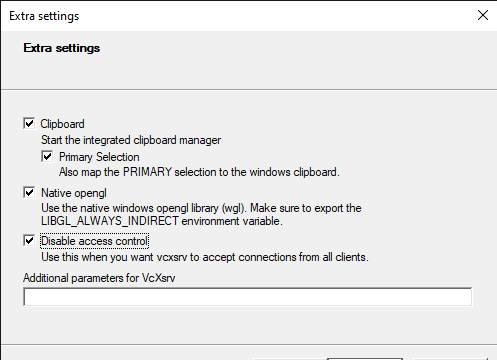
\includegraphics[scale=0.6]{vcxsrv_disable_access_control.png}
        \end{figure}
    \item Following \cite{alextsil2020steps}, go to Settings -\trangle Windows
        Defender Firewall -\trangle "Allow an app or feature through Windows
        Defender Firewall" and enable BOTH "VcXsrv windows xserver (X2Go/Arctica
        Builds) as seen in the screenshot below:
        \begin{figure}[H]
            \centering
            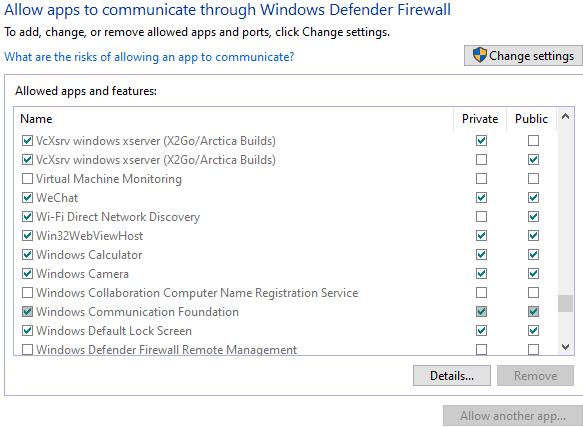
\includegraphics[scale=0.6]{vcxsrv_firewall.png}
        \end{figure}
    \item To test that VcXsrv now works, with Zathura installed, run "zathura
        name.pdf" and see if it opens.
\end{enumerate}
Note that the settings in Step 2 will revert itself. To accommodate for this,
you will be prompted in the next window to save the file "config.xlaunch". From
here, simply follow the instructions in Section \ref{SecAutostart} so that the
configuration is set after logging in.

%------------------------------------------------------------------------------
\subsection{Vimtex+Zathura+Synctex}
%------------------------------------------------------------------------------
Now you're almost ready to run Vimtex+Zathura+Synctex! You'll need to also
install xdotool by using "sudo apt-get install xdotool". To test whether this
works with VcXsrv following the suggestion in \cite{paulrougieux2020vimtex} from
lervag himself, run "xdotool search --class Zathura" and some numbers should
appear. From here, you should be good to go! Simply follow the steps laid out in
Section \ref{SecFwdBckwdSynctex}.\\

If this fails and you've given up on Zathura, you can alternatively use the
Sumatra PDF viewer. Once installed, simply add the following lines to your
vimrc:
\begin{lstlisting}
    let g:vimtex_view_general_viewer  = '/mnt/c/Users/Hwan/AppData/Local/SumatraPDF/SumatraPDF.exe'
    let g:vimtex_view_general_options = '-reuse-instance -forward-search @tex @line @pdf'
    let g:vimtex_view_general_options_latexmk = '-reuse-instance'
\end{lstlisting}
However, with this, you won't have access to forward and backward search via
synctex.

%==============================================================================
\section{Windows Terminal}
%==============================================================================
The default Ubuntu terminal is pretty trash. Instead, I recommend the `Windows
Terminal' which is highly customizable. Not only does it allow for multiple tabs
but each tab can run a different program i.e. the Linux bash as well as
PowerShell.\\

The customization can be done using the UI or via the \textbf{settings.json}
file which can be opened by clicking the cog displayed below:
\begin{figure}[H]
    \centering
    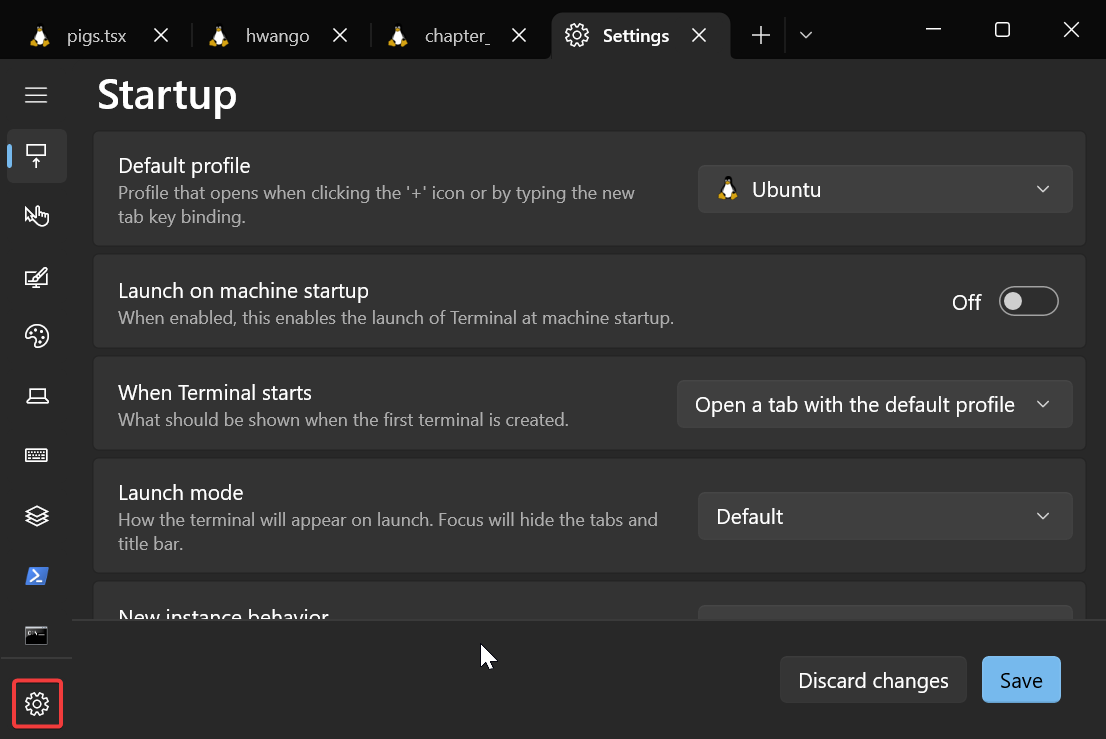
\includegraphics[scale=\figscale]{windows_terminal_settings_json.png}
    \caption{Click to open \textbf{settings.json} file.}
    \label{FigWindowsTerminalSettingsJSON}
\end{figure}
The file path to the file is:
\begin{lstlisting}
C:\Users\<Username>\AppData\Local\Packages\Microsoft.WindowsTerminal_8wekyb3d8bbwe\LocalState
\end{lstlisting}

%==============================================================================
\section{Troubleshooting}
%==============================================================================
%------------------------------------------------------------------------------
\subsection{Vim Display Issues on Startup}
%------------------------------------------------------------------------------
When using Windows Terminal, you may notice that Vim has display issues when
starting up. Specifically, the columns might appear `diagonally' and only
resolves itself after playing around with the window i.e. toggling full screen
on and off. This is because the following settings in your vimrc:
\begin{lstlisting}
    set lines=62 columns=120
\end{lstlisting}
garbles the initial startup of Vim in Windows Terminal. Simply disable this
setting and the issue will disappear as suggested by waf's answer in
\cite{tompounceonGit2020vim}.

%------------------------------------------------------------------------------
\subsection{Visual Block Mode}
%------------------------------------------------------------------------------
To enter visual block mode in Vim, you need to press `ctrl+V'. However, in
Windows, this is bound to paste. Therefore, open the Windows Terminal settings
and open the `settings.json' file. Then locate the following code:
\begin{lstlisting}
        {
            "command": "paste",
            "keys": "ctrl+v"
        },
\end{lstlisting}
and change it to `ctrl+shift+v' if you like to mimic Linux.

%------------------------------------------------------------------------------
\subsection{Clash with Anaconda}
%------------------------------------------------------------------------------
You may notice that after installing Anaconda, when using
Vimtex+Zathura+Synctex, you may get the error `vimtex cannot find zathura
windows id' and forward/backwards search does not work. With some
experimentation, I discovered that in your .bashrc, the following block of code
that is added automatically with the installation of Anaconda:
\begin{lstlisting}
# >>> conda initialize >>>
# !! Contents within this block are managed by 'conda init' !!
__conda_setup="$('/home/hwangoh/anaconda3/bin/conda' 'shell.bash' 'hook' 2> /dev/null)"
if [ $? -eq 0 ]; then
    eval "$__conda_setup"
else
    if [ -f "/home/hwangoh/anaconda3/etc/profile.d/conda.sh" ]; then
        . "/home/hwangoh/anaconda3/etc/profile.d/conda.sh"
    else
        export PATH="/home/hwangoh/anaconda3/bin:$PATH"
    fi
fi
# unset __conda_setup
# <<< conda initialize <<<
\end{lstlisting}
causes the issue. Specifically, I noticed that if I comment out the line:
\begin{lstlisting}
__conda_setup="$('/home/hwangoh/anaconda3/bin/conda' 'shell.bash' 'hook' 2> /dev/null)"
\end{lstlisting}
then everything works fine with Vimtex+Zathura+Synctex. However, the terminal
command `conda' no longer works. When that line is removed, one no longer has
`(base)' at the beginning of each line in the terminal, so I suspect that there
is some clash with the anaconda environment. Therefore, a workaround follows
from \cite{drylabrebel2019how} where the answers suggest to run the
following command in terminal:
\begin{lstlisting}
conda config --set auto_activate_base false
\end{lstlisting}
which ensures that the Anaconda base envionment does not automatically appear by
default when the terminal is started.\\

This generally seems to fix the problem. However, I noticed that when compiling
tex documents using the LaTeX template used to write these notes, I get the
error `Compilation failed'. Despite this, you can still use `VimtexView' to open the
pdf and notice that compilation does work as the pdf does change. Additionally,
forward and backward search works as well. So I just ignore the error.

%------------------------------------------------------------------------------
\subsection{Localhost Errors}
%------------------------------------------------------------------------------
Often in web development, one would need start a server on localhost for local
development. However, with WSL2, this sometimes fails. To remedy this issue,
following \cite{reescarter2020wsl2}, we need to disable the `Fast Start-Up'
option:
\begin{enumerate}
    \item First navigate to control panel and select `System':
        \begin{figure}[H]
            \centering
            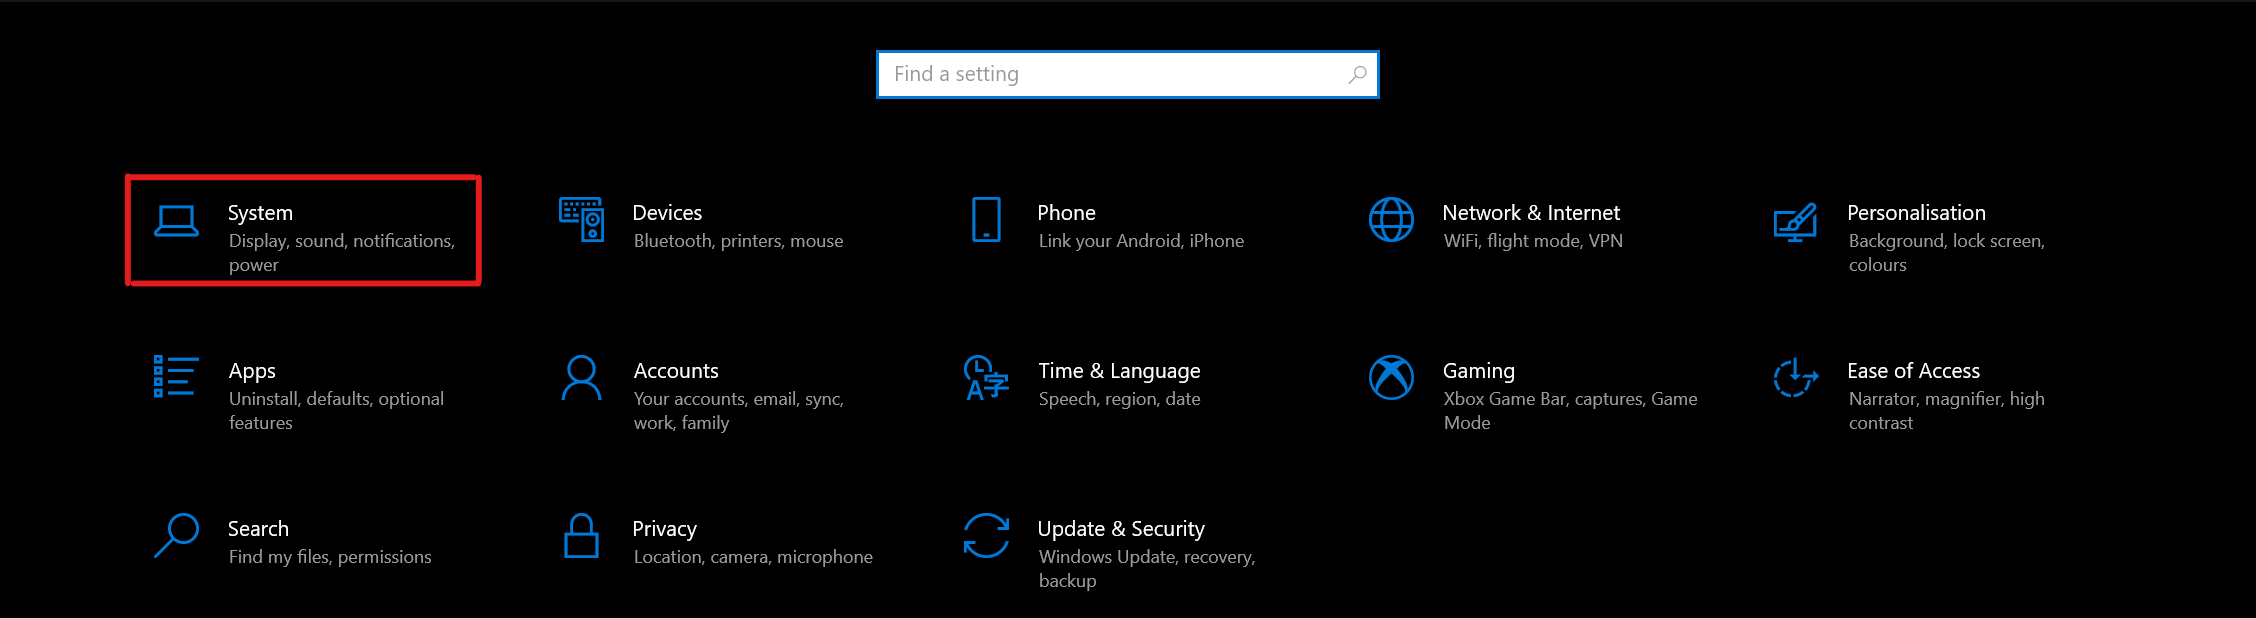
\includegraphics[scale=\figscale]{windows_settings_system.png}
            \caption{Windows settings: `system'}
            \label{FigWindowsSettingsSystem}
        \end{figure}
    \item Navigate to `Power \& sleep' on the left-blade and select `additional
        power settings':
        \begin{figure}[H]
            \centering
            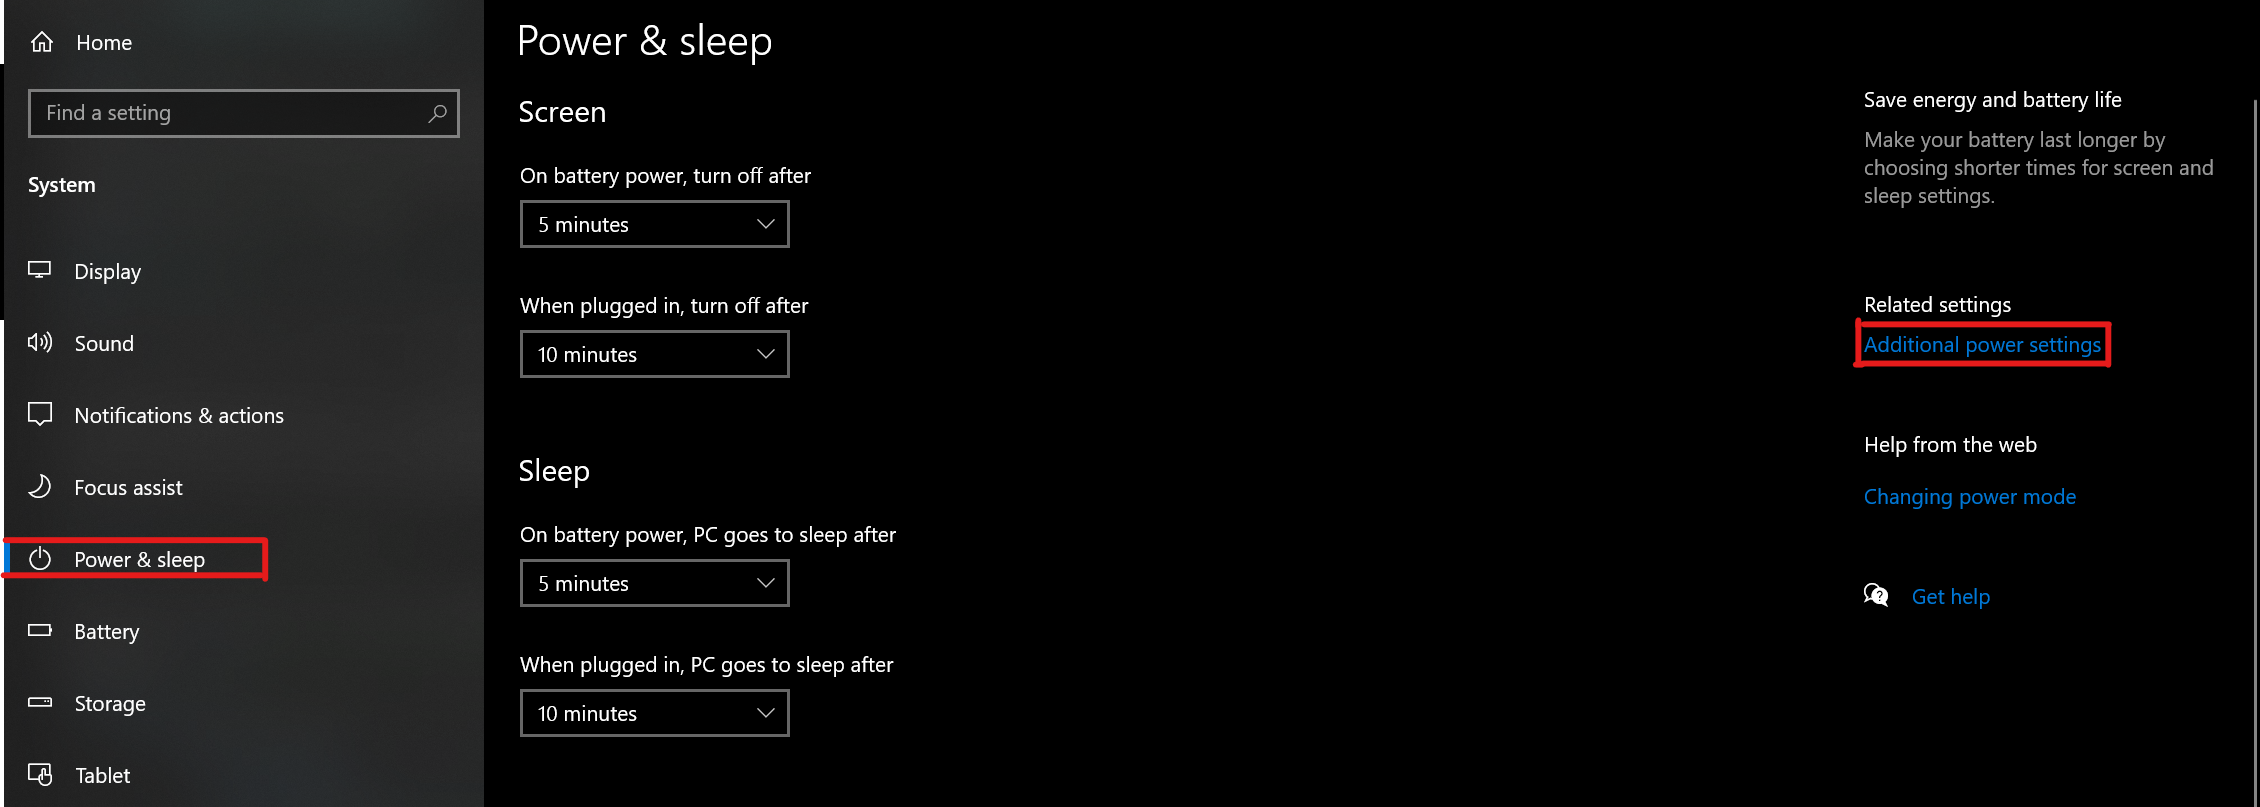
\includegraphics[scale=\figscale]{windows_settings_additional_power_settings.png}
            \caption{Windows settings: additional power settings}
            \label{FigAdditionalPowerSettings}
        \end{figure}
    \item Select `Choose what the power button does':
        \begin{figure}[H]
            \centering
            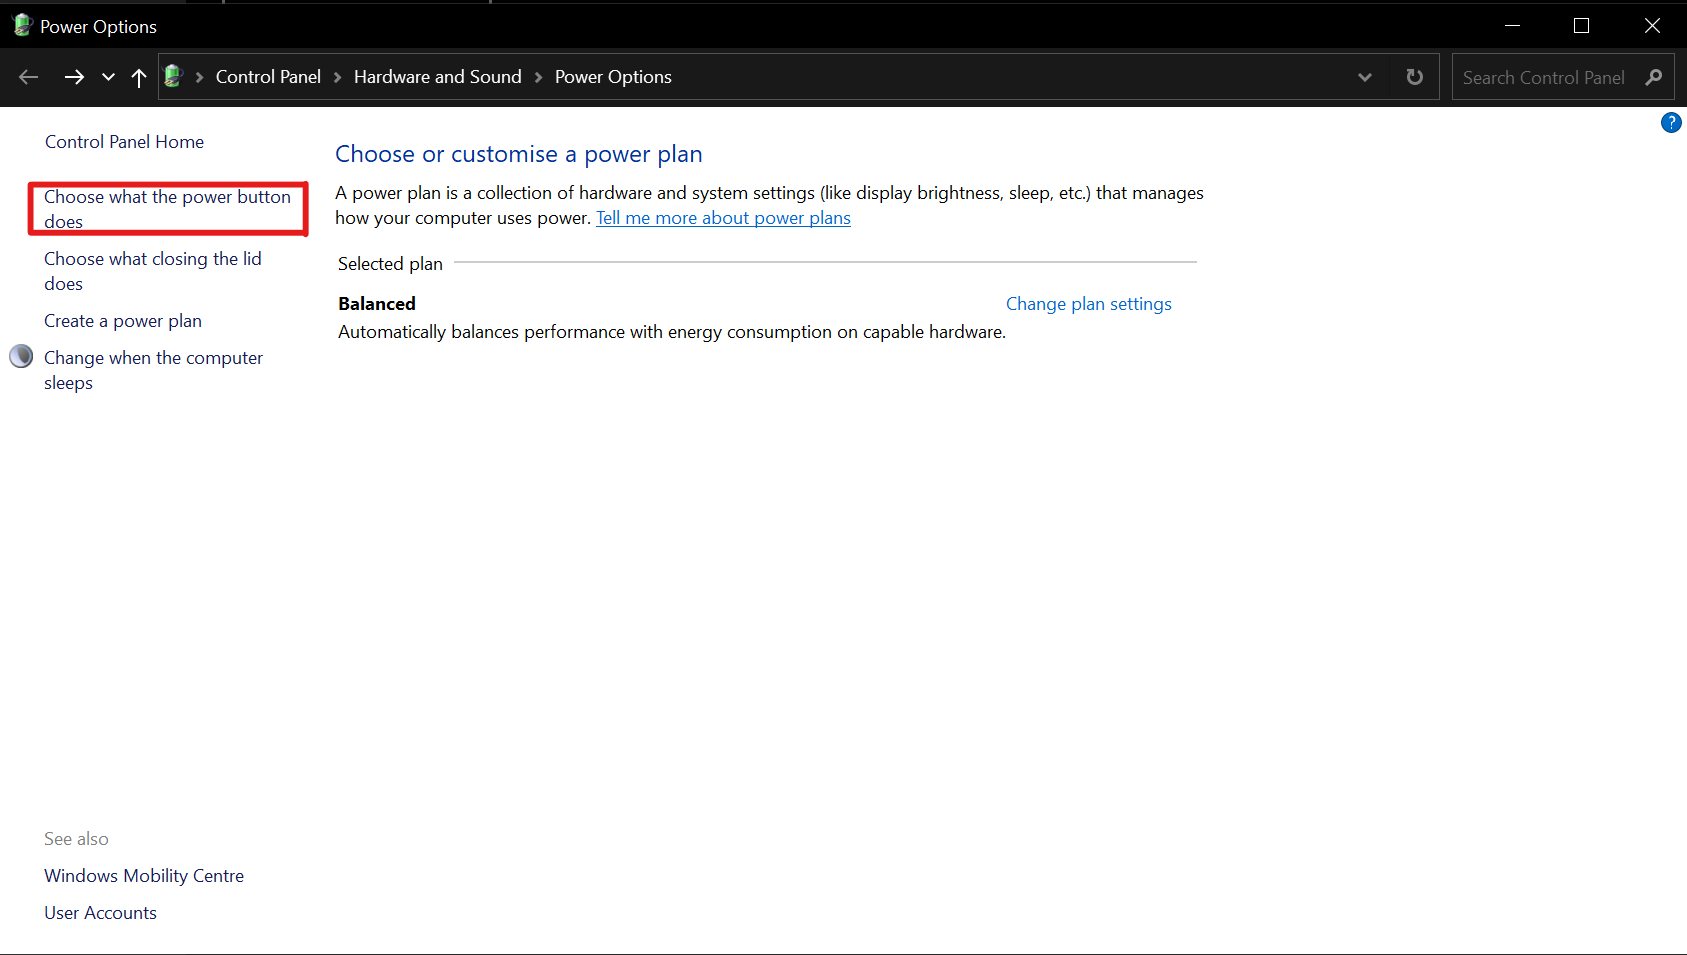
\includegraphics[scale=\figscale]{windows_settings_choose_what_the_power_button_does.png}
            \caption{Windows settings: choose what the power button does}
            \label{FigChoosePowerButton}
        \end{figure}
    \item Then select `Change settings that are currently unavailable' to allow
        administration privileges to alter settings. Then uncheck the checkbox
        for `Turn on fast start-up':
        \begin{figure}[H]
            \centering
            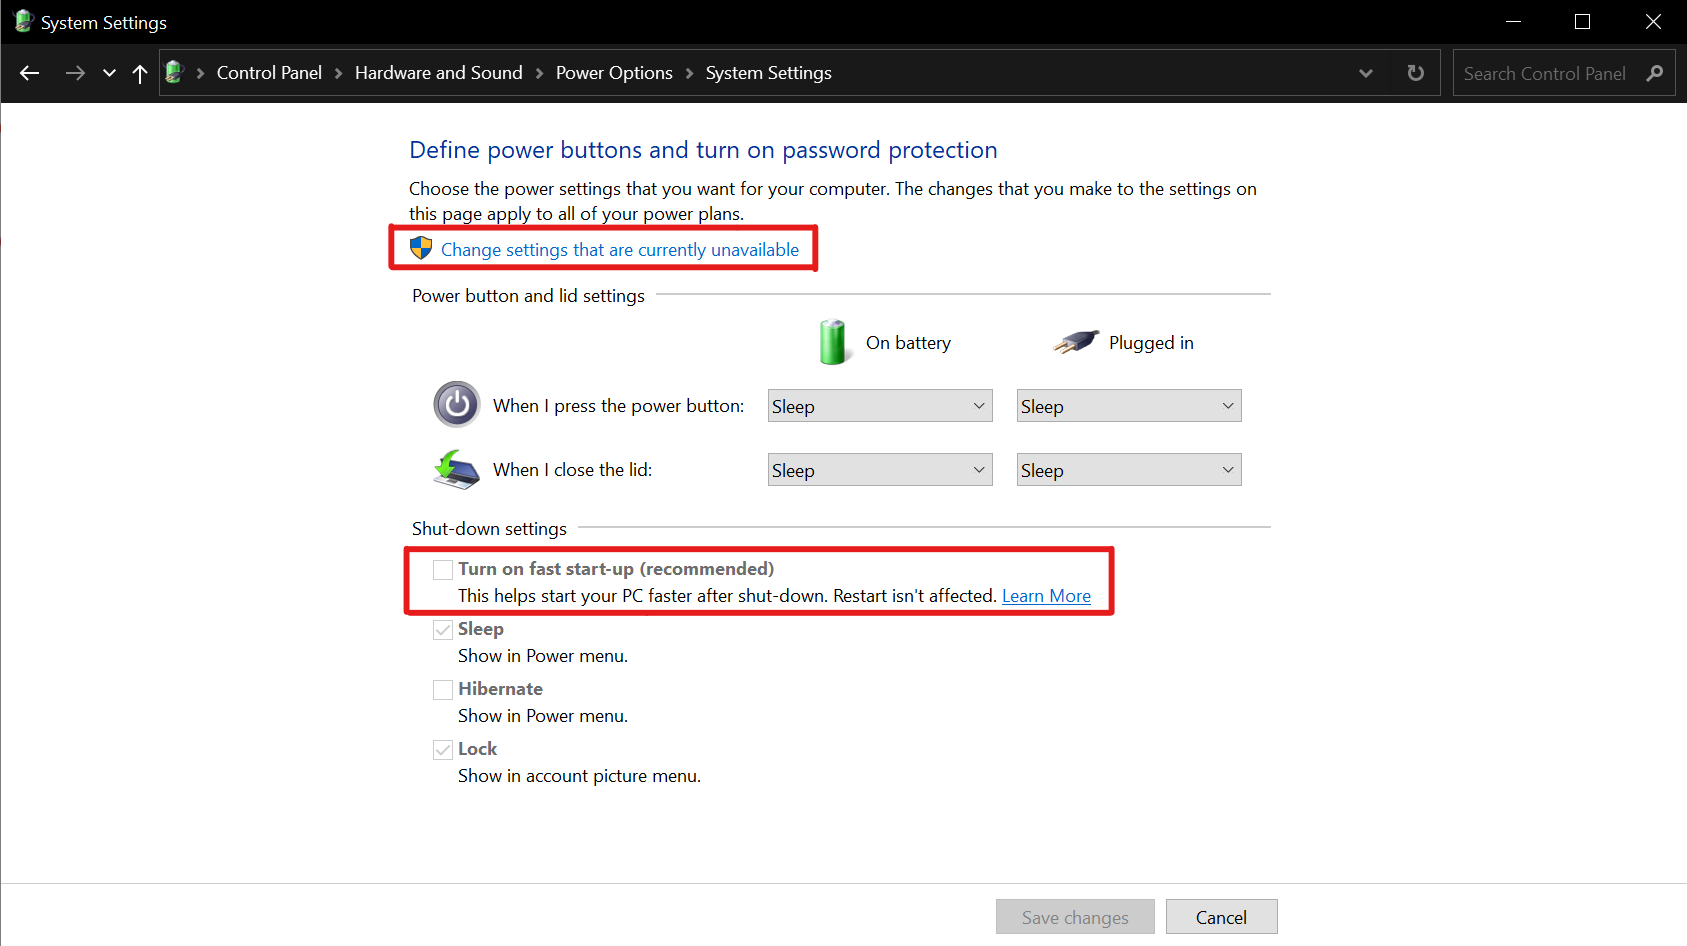
\includegraphics[scale=\figscale]{windows_settings_turn_on_fast_start_up.png}
            \caption{Windows settings: turn on fast startup}
            \label{FigTurnOnFastStartUp}
        \end{figure}
    \item Restart your computer
\end{enumerate}


\chapter{Miscellaneous} \label{ChapMisc}

%==============================================================================
\section{.bashrc Stuff}
%==============================================================================
%------------------------------------------------------------------------------
\subsection{Run \textbf{ls} after \textbf{cd}}
%------------------------------------------------------------------------------
Following `frabjous' answer to the StackOverflow question
\cite{robkohr2011make}, you can add the following to your .bashrc:
\begin{lstlisting}
function cd {
    builtin cd "$@" && ls -F
}
\end{lstlisting}
He also mentions that he adds
\begin{lstlisting}
    [ -z "$PS1" ] && return
\end{lstlisting}
before this so that ``everything after that line only applies to interactive
sessions, so this doesn't affect how \textbf{cd} behaves in scripts." How this
works is also explained by him:\\
``$[ -z "\$PS1" $] checks if the \$PS (interactive prompt variable) is `zero
length' (-z). If it is zero length, this means it has not been set, so Bash must
not be running in interactive mode. The \&\& return part exits from sourcing
.bashrc at this point, under these conditions."

%==============================================================================
\section{Ranger}
%==============================================================================
Following \cite{linuxcompendium2019ranger}:
\begin{enumerate}
    \item git clone https://github.com/hut/ranger.git
    \item cd ranger
    \item sudo make install
\end{enumerate}
To start ranger use "ranger".

%------------------------------------------------------------------------------
\subsection{Configuration}
%------------------------------------------------------------------------------
After the configuration directory has been created by the Ranger, you can now copy its configuration files by running the following commands in terminal:
\begin{itemize}
    \item "ranger --copy-config=all". Now you can run "cd ~/.config/ranger" to see the
        configuration files.
\end{itemize}

%==============================================================================
\section{Inkdrop}
%==============================================================================
\emph{Inkdrop} \cite{matsuyamainkdrop} is an absolutely incredible minimalist and
light-weight markdown-based note taking app that syncs across all devices.
It is a paid service of around \$5 a month or \$50 a year should you chose to
pay annually. It also has a convenient plugin GUI which can be accessed via the
settings menu. Since the creator is a Vim user, there is of course a Vim
plugin:
\begin{figure}[H]
    \centering
    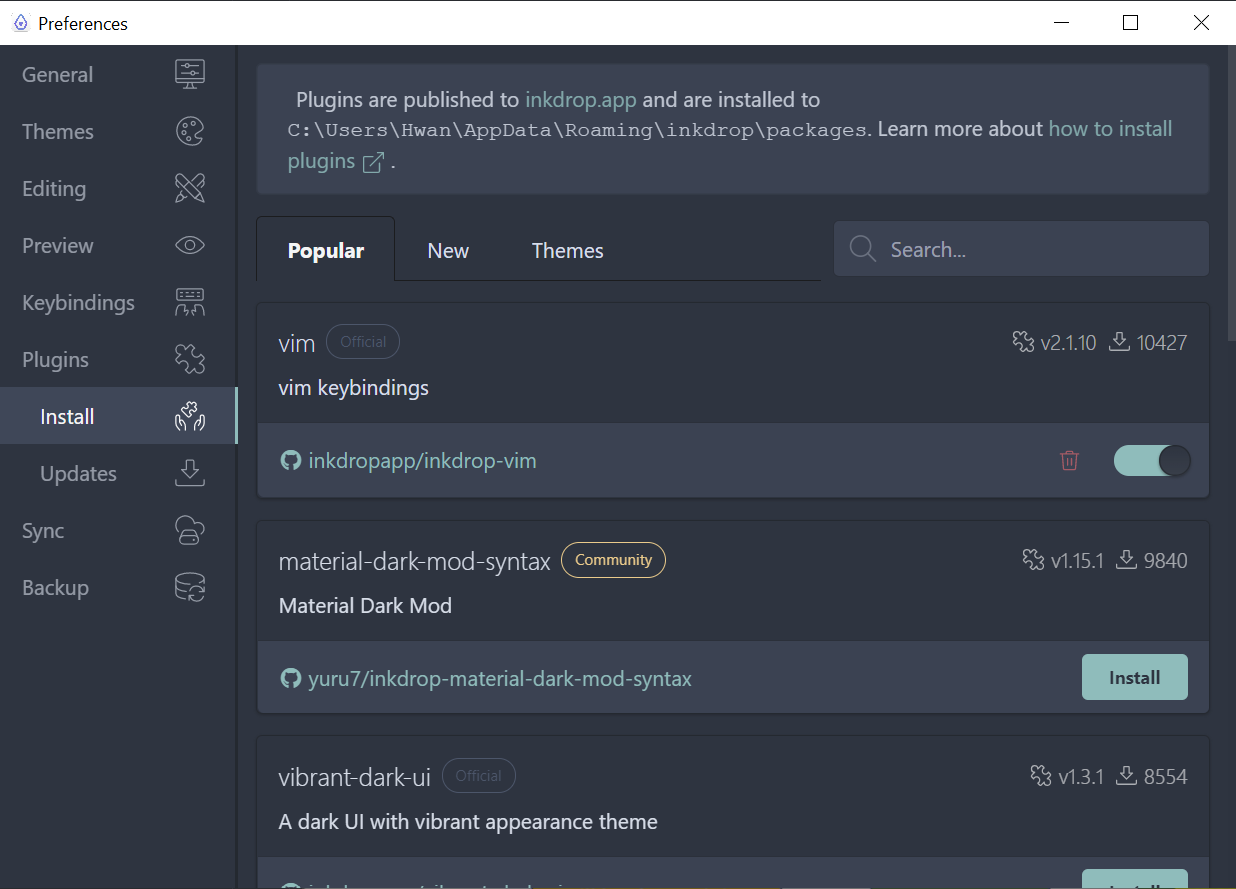
\includegraphics[scale=\figscale]{Figures/inkdrop_vim_plugin.png}
    \caption{Inkdrop Vim plugin}
    \label{FigInkdropVimPlugin}
\end{figure}
To modify the key bindings, following the Inkdrop user manual
\cite{matsuyamacustomizing} you can modify the \textbf{keymap.cson} file which
can be instantly directed to using the following link:
\begin{figure}[H]
    \centering
    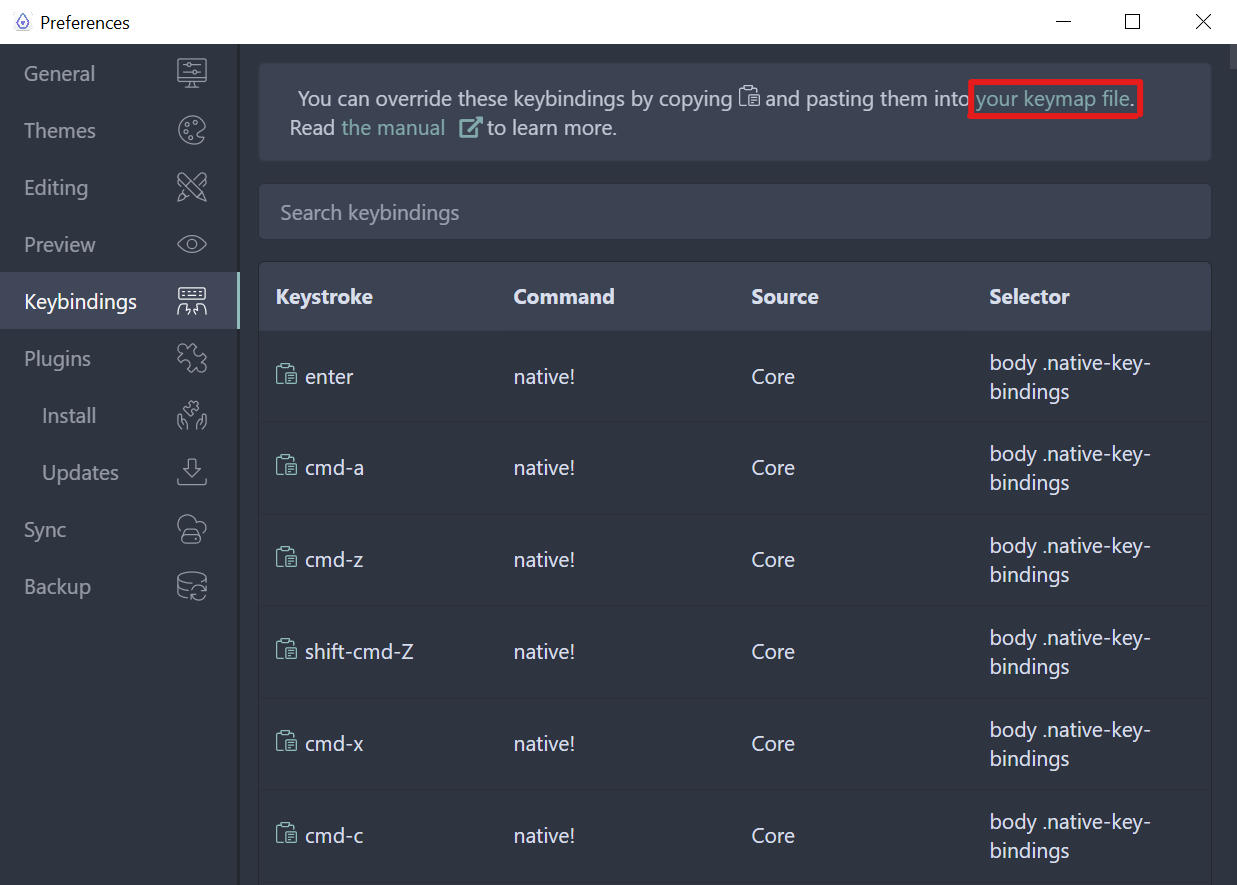
\includegraphics[scale=\figscale]{Figures/inkdrop_keymap_file.png}
    \caption{Inkdrop keymap file link}
    \label{FigInkdropKeymapFile}
\end{figure}
Here is an example of the \textbf{keymap.cson} file:
\begin{lstlisting}
'.CodeMirror.vim-mode:not(.insert-mode):not(.key-buffering) textarea':
  'shift-j': 'vim:scroll-down'
  'shift-k': 'vim:scroll-up'
  'ctrl-j': 'vim:join'
\end{lstlisting}
You can modify this in Vim after navigating to it in terminal and with Inkdrop
on. Any saved changes will be instantly reflected in the app and errors will
result in a popup.


\cleardoublepage \phantomsection

%---------------------------------------------------------------
%:                  BACK MATTER:  Bibliography
% --------------------------------------------------------------
\nocite{*}
\bibliography{references}{}
\bibliographystyle{abbrv}
%---------------------------------------------------------------
%        END: Bibliography
%---------------------------------------------------------------

\end{document}
